% !TeX root = ../thesis.tex

% \documentclass[12pt]{article}
% % packages used
% \usepackage{geometry}
% \usepackage{amsmath}
% \usepackage{amssymb}
% %\usepackage{amsfonts}
% \usepackage{amsthm}
% \usepackage{bm}
% \usepackage{graphicx}
% \usepackage{cite}

% % fonts used
% %\usepackage{fourier}
% %\usepackage{fourier}
% %\usepackage{nimbusmononarrow}
% \usepackage{microtype}
% %\usepackage{fontspec}
% %\setsansfont{Linux Biolinum}
% %\setmonofont{Linux Mono}
% % theorems, remarks, etc
%   %% types italiques
% \theoremstyle{plain}
% \newtheorem{lemma}{Lemma}[section]
% \newtheorem{proposition}{Proposition}[section]
% \newtheorem{theo}{Theorem}[section]
% \newtheorem{algo}{Algorithm}[section]
% \newtheorem{assump}{\bf{Assumption}}[section]
% \newtheorem{conj}{Conjecture}[section]
%   %% types roman
% \theoremstyle{remark}
% \newtheorem{remark}{\bf{Remark}}[section]
% \theoremstyle{remark}
% \newtheorem{example}{\bf{Example}}[section]
% \theoremstyle{remark}
% \newtheorem{definition}{\bf{Definition}}[section]
  %\newtheorem{appendix}{\bm Definition}[section]

%------------------------------------------------------------------------
%--------------------------- personal macros ---------------------------
%------------------------------------------------------------------------

%\renewcommand{\theequation}{\arabic{section}.\arabic{equation}}
%\numberwithin{equation}{section}

\newcommand*\diff{\mathop{}\!\mathrm{d}}
\newcommand*\Diff[1]{\mathop{}\!\mathrm{d^#1}}

%----- typos
\newcommand{\ie}{{\it i.e. \/}}

%----- fractions
\newcommand{\half}{\frac{1}{2}}

%---- bold characters
\newcommand{\bx}{{\bf{x}}}
\newcommand{\by}{{\bf{y}}}
\newcommand{\bk}{{\bf{k}}}
\newcommand{\bz}{{\bf{0}}}

%----- set
\newcommand{\R}{{\mathbb{R}}}
\newcommand{\Z}{{\mathbb{Z}}}
\renewcommand{\N}{{\mathbb{N}}}
\newcommand{\Nm}{{\mathcal{N}}}
\renewcommand{\RN}{\R^{\N}}
\newcommand{\p}{\mathcal{P}}

%----- derivatives
\newcommand{\dt}{\partial_t}
\newcommand{\dx}{\partial_x}
\newcommand{\dxx}{\partial_{xx}}
\newcommand{\dyy}{\partial_{yy}}
\newcommand{\dtt}{\partial_{tt}}
\newcommand{\dtx}{\partial_{tx}}
\newcommand{\dxtt}{\partial_{xtt}}
\newcommand{\dtxx}{\partial_{txx}}
\newcommand{\grdx}{\nabla_x}

\renewcommand{\dz}{\partial_z}
\newcommand{\dnz}[1]{\partial^{#1}_z}

%----- greek letters
\newcommand{\eps}{\varepsilon}

%----- initial model
\newcommand{\av}[1]{\left[ #1 \right]}

%----- numerical scheme
\newcommand{\Dx}{\Delta x}
\newcommand{\Dt}{\Delta t}
\newcommand{\Dv}{\Delta v}

\newcommand{\tn}{t^n}
\newcommand{\tnp}{t^{n+1}}
\newcommand{\x}{x_i}
\newcommand{\xp}{x_{i+1}}
\newcommand{\xpd}{x_{i+\half}}

\newcommand{\Uniz}{U^n_i(z)}
\newcommand{\Unpiz}{U^{n+1}_i(z)}
\newcommand{\Unimz}{U^n_{i-1}(z)}
\newcommand{\Unik}{U^n_{i,(k)}}
\newcommand{\UniK}{U^n_{i,(K)}}
\newcommand{\hUnpi}{\hat{U}^{n+1}_i}
\newcommand{\bhUnpi}{\hat{\bm{U}}_i^{n+1}}
\newcommand{\hUni}{\hat{U}^n_i}
\newcommand{\bhUni}{\hat{\bm{U}}^n_i}

\newcommand{\hUnim}{\hat{U}^n_{i-1}}
\newcommand{\bhUnim}{\hat{\bm{U}}^n_{i-1}}
\newcommand{\hUnik}{\hat{U}^n_{i,(k)}}

\newcommand{\lp}{\lambda^+}
\newcommand{\lm}{\lambda^-}
\newcommand{\lpm}{\lambda^{\pm}}
\newcommand{\lpmz}{\lambda^{\pm}(z)}
\newcommand{\lpz}{\lambda^+(z)}
\newcommand{\lmz}{\lambda^-(z)}


%------------------------------------------------------------------------
%----------------------- end of personal macros ------------------------
%------------------------------------------------------------------------


% \begin{document}

% % \begin{flushright}
% %   {\it draft, \today}
% % \end{flushright}
% %\begin{center}
% \title{\bf The Discrete Stochastic Galerkin Method for Hyperbolic Equations
% with Non-smooth and Random Coefficients\footnote{This research was supported by NSFC grant No. 91330203, NSF
% grants DMS-1522184 and DMS-1107291: RNMS KI-Net, and by the Office
% of the Vice Chancellor for Research and Graduate Education at the University of Wisconsin-Madison with
% funding from the Wisconsin Alumni Research Foundation.}}

% \vspace{1cm}
% \author{Shi Jin\footnote{ Institute of Natural Sciences, Department of Mathematics, MOE-LSEC and SHL-MAC, Shanghai Jiao Tong University, Shanghai 200240, China and Department of Mathematics, University of Wisconsin-Madison, Madison, WI 53706, USA (jin@math.wisc.edu) and .} \ and Zheng Ma\footnote{Department of Mathematics, Shanghai Jiao Tong University, Shanghai 200240, China.}}
% %\end{center}

% \maketitle

% \begin{abstract}
% \noindent 
% We develop a general polynomial chaos (gPC) based stochastic Galerkin (SG) for
% hyperbolic equations with random and singular coefficients. Due to the singular nature of the solution, the standard gPC-SG methods may suffer from a poor or even
% non convergence. Taking advantage of the fact that the discrete solution,
% by the central type  finite difference or finite volume approximations
% in space and time for example, 
% is smoother, we first discretize the equation by a smooth finite difference or
% finite volume scheme, and then use the gPC-SG approximation to the discrete
% system. The jump condition at the interface is treated using the immersed
% upwind methods introduced in \citen{Jin:2009pro, Wen:2005ueba}.
% This yields a method that converges with the spectral accuracy
% for finite mesh size and time step.  We use a linear hyperbolic equation
% with discontinuous and random coefficient, and the Liouville equation with
% discontinuous and random potential, to illustrate our idea, with both one
% and second order spatial discretizations. Spectral convergence is established 
% for the first equation, and numerical examples for both equations show the
% desired accuracy of the method.

% \bigskip

% \noindent{\bf Key words.} hyperbolic equation, random coefficient, potential barrier, stochastic Galerkin, polynomial chaos\\
% {\bf AMS subject classifications.} 35L02, 65M06, 65M60, 65C30\\
% \end{abstract}
\chapter{gPC-SG方法在带有间断及随机系数的双曲型方程中的应用}

%--------------------------------------------------------------------------
%\section{简介}
%\label{intro}
%--------------------------------------------------------------------------
%In this report, I will summarize some new results and understanding on the one dimension convection equation with discontinuous and random speed.
% We are interested in developing efficient numerical methods to solve
% linear hyperbolic equations with non-smooth and uncertain coefficients. Such problems arise in wave propagation in heterogeneous media, through interfaces between different media, or potential barriers,  making the coefficients in
% these equations discontinuous or even more singular. Random uncertainties arise
% due to modeling or experiment errors. These errors are inevitable since the
% fluxes in  hyperbolic equations are often given by {\it empirical} laws, equations of state or
% moment closures which are often {\it ad hoc}.

我们的目标是发展有效的数值方法来解决具有不光滑和不确定系数的线性双曲型方程。这样的问题通常出现在异质介质中的波传播中,由于不同介质之间具有界面或势垒,方程出现间断或甚至更很强的奇异性。而随机或不确定性的出现则是由于建模或实验中的误差,由于双曲方程中的通量通常是由{\it 经验定律}、状态方程或矩封闭方法给出,导致了这种误差{\it 非常特殊},通常无法通过其他手段去掉或者减小。

% When hyperbolic equations contain singular coefficients, one usually needs to
% provide an extra physical condition at the singular points to make the 
% initial or boundary value problems well-posed and to account for 
% the correct physics of waves at the interface or barrier\citen{Wen:2005ueba, Jin:2009pro}.
% In the case of potential barriers, a natural physical condition is the transmission
% and reflection conditions,  and such conditions
% can be built into the numerical fluxes in a natural way, in the framework of
% the Hamiltonian-Preserving schemes\citen{Wen:2005ueba, JinWen-wave}. 
% This is the approach we will take to tackle the problems with singular coefficients.

当双曲方程包含奇异系数时,通常需要在奇异点提供额外的物理条件以使得初边界值问题是适定的,同时能够反应在界面或势垒处的波的正确物理行为\citen{Wen:2005ueba, Jin:2009pro}。在势垒的情况下,一个自然的物理条件就是折射和反射条件,在所谓的哈密尔顿守恒格式(Hamiltonian-Preserving)的框架中\citen{Wen:2005ueba, JinWen-wave},这些条件可以自然的构建到数值格式的通量中。这是我们将采用的解决奇异系数引起的困难的方法。

% To handle the difficulty induced by the random uncertainties, we will utilize the generalized
% polynomial chaos (gPC) expansion based stochastic Galerkin (SG) method\citen{Bijl:2013hkba, GS, GWZ, LMK, PIN, Tryoen:2010djba, Xiu:2010wxba, XiuKar}.
% Such methods outperform the classical Monte-Carlo method in that, given
% sufficient regularity of the solution in the random space, they can achieve
% the spectral convergence, thus are  much more efficient  for
% problems with random uncertainties. Unfortunately, for hyperbolic problems,
% one often is not blessed with such regularities, which leads to 
% significant reduction of order of
% convergence\citen{Motamed:2012gsba, Tang:2012ibba},
%  thus slows down the computation or even gives 
% non-convergent results due to Gibbs' phenomenon.  The problems under study in this paper are  problems with discontinuous solutions in the random space, due to jumps of solutions formed at the interfaces or barriers which will propagate
% into the random space.

为了处理由随机不确定性带来的困难,我们将利用广义多项式混沌(generalized Polynomial Chaos (gPC))展开为基础的随机伽辽金(stochastic Galerkin (SG))方法\citen{Bijl:2013hkba, GS, GWZ, LMK, PIN, Tryoen:2010djba, Xiu:2010wxba, XiuKar}。如果方程的解在随机空间具有足够的正则性,这种方法实现谱收敛,远快于经典的蒙特卡罗方法,因此对于这种随机不确定性的问题更有效率
。不幸的是,对于双曲型问题,解经常不会有这样好的正则性,这导致方法收敛的速度非常缓慢甚至给出由于吉布斯现象导致的非收敛结果\citen{Motamed:2012gsba,Tang:2012ibba}。本章中研究的对象就是由于在物理空间的界面、势垒导致的解的跳跃、间断,随之波动方程的演化而传播到随机空间,从而导致解在随机空间具有很差的光滑性的一类问题。

% A standard gPC-SG method begins with a gPC approximation of the original
% differential equation in the random space,  yielding a {\it deterministic} system of equations
% for the gPC coefficients (while the randomness is built into the
% basis functions which are orthonormal polynomials), which is then discretized
% by standard schemes (finite difference, finite volume, finite element, or
% spectral methods) in space and time. The gPC approximation
% is accurate if solutions to the original problem are smooth in the random
% space. This is not the case for the problems under study.

标准的gPC-SG方法过程如下:先对原始的微分方程在随机空间做gPC逼近(随机空间的正交多项式逼近),这样会得到一个关于gPC展开系数的{\it 确定性的}方程组(而随机性蕴含在gPC正交多项式的基函数)。然后再用通常的方法将其空间和时间数值离散化(有限差分,有限体积,有限元或谱方法)。如果原始问题的解在随机空间是充分光滑的,那么这种gPC逼近方法是非常准确的。不幸的是,我们研究的问题恰恰不属于这种情况。

% Our central idea in this paper is to {\it reverse} the above gPC-SG process.  Namely,
% we first discretize the original equation in space and time, using {\it smooth} numerical fluxes, and then apply the gPC approximation to this discrete
% equation.  Since the discrete solution is more regular than the continuous one,
% the gPC approximation is applied to a smoother function (for fixed time step
% and mesh  size), thus one expects a better convergence rate. We refer to
% such gPC-SG methods as the {\it discrete gPC-SG methods}.

本章中我们的主要思想是{\it 逆转}上述gPC-SG过程。也就是说,我们首先使用{\it 光滑的}数值通量在空间和时间上对原始方程进行离散,然后再将gPC近似应用于该离散方程。由于离散后的数值解解比原连续方程的解具有更好的正则性,gPC逼近则应用于该光滑的函数(对于固定的时间步长和网格大小),因此可以期望有更好的收敛速度。我们称这样的gPC-SG方法为{\it 离散gPC-SG方法}。在\citen{Motamed:2012gsba}的随机配点法的框架下,提出并分析了一个类似的想法,他们也注意到,虽然解确实是不连续的,但是一些人们感兴趣的量(quantities of interests, QoI)通常具有更好的正则性,从而可以期待更好的收敛速度。

% For hyperbolic equations, the smooth numerical fluxes are usually
% central differences which do not depend on the characteristic information (for examples the Lax-Friedrichs, the Lax-Wendroff scheme, 
% etc.). The upwind type schemes are not smooth, since they depend on the sign of
%  the absolute value of the characteristic speeds thus do not yield smooth 
% numerical fluxes.
%  For second order scheme, in order to
% suppress numerical viscosity, one usually uses slope limiters or ENO or
% WENO type reconstruction\citen{LeVeque, Tadmor:2000jlba, Tadmor:1990vlba} which in general are not smooth functions.
% In order to keep the numerical flux smooth, we use the smooth BAP slope limiter
% introduced in\citen{Liu:1998faba}.

对于双曲型方程,光滑的数值通量通常由中心差分得到,因为中心差分格式不依赖于特征线的信息(例如Lax-Friedrichs格式,Lax-Wendroff格式,等等)。而迎风类型的格式则通常会导致不光滑的数值通量,因为它们依赖于于特征线传播速度的绝对值。对于二阶(或高阶)格式,为了抑制数值粘性,通常使用斜率限制器(slope limiter或者flux limiter)或ENO或
WENO型重构\citen{LeVeque, Tadmor:2000jlba, Tadmor:1990vlba},而其通常不是光滑函数。为了保持数值通量光滑,我们使用文章\citen{Liu:1998faba}中引入的光滑的BAP斜率限制器。

% In this paper we will develop this idea for two problems. The first
% is a scalar hyperbolic equation with a discontinuous and random coefficient:
在本章中,我们将用这个新想法的来研究两个问题。首先是具有间断和随机系数的标量双曲型方程:
\begin{equation}
\label{conv-eq}
  u_t(x, t, z) + \big[c(x,z)u(x,t,z)\big]_x = 0, \quad t > 0.
\end{equation}
% Here $c(x,z)$ is the random coefficient where $z$ is a random variable in a properly defined complete random space with event space $\Omega$ and probability distribution function $\rho(z)$. $c(x,z)$ is discontinuous respect to $x$, which corresponds to an interface between different media. The second is the Liouville equation for the particle density distribution $u(x,t,z)>0$:
这里$c(x,z)$是随机系数(随机波速),其中$z$是在完备样本空间$\Omega$中概率密度分布函数为$\rho(z)$的随机变量。$c(x,z)$关于$x$是简短的,这对应于不同介质之间的界面。第二个问题是是粒子密度分布$u(x,v,t,z)>0$的刘维尔(Liouville)方程:
\begin{equation}\label{eq_Liou}
  u_t + v  u_x - V_x  u_v = 0, \quad t>0, \quad x, v \in \R,
\end{equation}
% in which the potential function $V(x,z)$ may be discontinuous in $x$, corresponding to a potential barrier. 
% The quantities of interest to be computed in these problems include the expectation of $u$,
其中势函数$V(x,z)$关于$x$中是不连续的,这对应于一个势垒的情形。在这些问题中我们感兴趣的量包括$u$的期望值,
\begin{equation}\label{exp}
  \mathbb{E}[u] = \int u(z) \rho(z)\diff z.
\end{equation}
% and its variance
和方差
\begin{equation}\label{var}
  \mathbb{V}[u]:=\mathbb{E}\big[(u-\mathbb{E}(u))^2\big] = \int u(z)^2  \rho(z) \diff z - (\mathbb{E}[u])^2
\end{equation}

% For equation(\ref{conv-eq}), by using the Lax-Friedrichs scheme followed
% by the gPC-SG approximation,  we will establish the regularity and consequently the spectral convergence of the proposed method in
% the random space, while the numerical convergence in space and time is the
% same as the deterministic problem established in\citen{Qi:2013byba}.
% The error will be verified numerically, for both the convection and the Liouville equations. 

对于方程(\ref{conv-eq}),通过先使用Lax-Friedrichs格式再应用gPC-SG方法,我们将建立所提出的方法的正则性结果以及由此带来的在随机空间的谱收敛结果,而空间和时间的数值收敛是与在\citen{Qi:2013byba}中建立的确定性问题的分析类似。对于这些分析结果,我们都会给出相应的数值验证。

% In such problems the uncertainty may also come from the initial data. This is
% a well-studied problem\citen{GX, Tang:2012ibba} and our method can obviously be used in this case.

在这些问题中,不确定性也可能来自初始数据。这是个问题已经在文章\citen{GX, Tang:2012ibba}中给出了仔细的分析,我们的方法显然可以在这种情况下使用。

% The paper is organized as follows. In Section 2, we will present the
% discrete gPC-SG method for  the convection equation(\ref{conv-eq}),
% and conduct the regularity and numerical convergence analysis for the fully
% discrete scheme.  In Section 3, we will show how to use this idea for the Liouville equation for both first  and  second order spatial discretizations.
%  In Section 4, we will present numerical examples for both equations that will show an exponential convergence in the random space. 

本章的结构如下。在\ref{c2-2}节中,我们将介绍离散gPC-SG方法应用于对流方程(\ref{conv-eq}),并进行完整的正则性和全离散格式的数值收敛分析。在\ref{c2-3}节中,我们将展示如何将这个想法用于一阶和二阶空间离散的刘维尔方程。
在\ref{c2-4}节中,我们将给出对应于这两个方程的数值示例,它们将证实该方法在随机空间的谱收敛。


%--------------------------------------------------------------------------
\section{带有间断、随机波速的对流方程的离散gPC-SG方法}\label{c2-2}
%--------------------------------------------------------------------------

%In this section, We will introduce the discretized gPC scheme for this discontinuous, random convection equation. We will first consider the deterministic case as a validation of this method and then use gPC expansions to solve stochastic case.

% We first consider a scalar model convection equation
我们考虑如下的标量对流方程模型
\begin{equation}\label{eq:convection}
  \left\{
  \begin{aligned}
    &u_t(x,t,z) + \big[c(x,z)u(x,t,z)\big]_x = 0,\quad t>0, \\
    &u(x, 0, z) = u_0(x, z).
  \end{aligned}
  \right.
\end{equation}
% Here we consider the case that $c(x, z)$ can be discontinuous with respect to $x$ at some point, for example,
这里$c(x, z)$关于$x$在某些地方是间断的,例如,
\begin{equation}
  c(x, z) = 
  \begin{cases}
    c^-(z)>0, & \text{如果$x<0$}, \\
    c^+(z)>0, & \text{如果$x>0$}.
  \end{cases}
\end{equation}
% As in \citen{Jin:2009pro}, an interface condition at $x = 0$ is needed to make the problem well-posed:
根据文章\citen{Jin:2009pro},我们需要在$x = 0$处给一个界面条件使得整个问题是适定的:
\begin{equation}\label{interface_1}
  u(0^-,t, z) = \alpha(z)u(0^+,t,z).
\end{equation}
% where $\alpha(z) = 1$ corresponds to conservation of mass or $\alpha(z) = c^-(z) / c^+(z)$ for the conservation of flux which is the case we will use in the sequel. Notice that here we assume $c(x,z)$ is smooth enough with respect to the random variable $z$, and only has one discontinuous point at $x = 0$.
其中$\alpha(z) = 1$对应于质量守恒定律,而对于通量的守恒定义为$\alpha(z) = c^-(z) / c^+(z)$,后者是我们在本章中要考虑的情形。注意,这里我们假设$c(x,z)$关于随机变量$z$足够光滑,并且只有一个不连续点位于$x = 0$。

% The discontinuity of $u(x,t,z)$ generated by the interface condition (\ref{interface_1}) will propagate into the random space, preventing the gPC method from high order convergence due to Gibb's phenomenon. Here we propose a slightly different approach from the traditional gPC method: We first discretize equation (\ref{eq:convection}) in space and time as done in\citen{Qi:2013byba} with the random variable $z$ as a fixed parameter. A key idea in\citen{Qi:2013byba} is to ``immerse'' the interface condition(\ref{interface_1}) into the scheme. The gPC method will then be applied to the discrete system.
由于界面条件(\ref{interface_1})导致的$u(x,t,z)$的间断将从物理空间传播到随机空间,带来的吉布斯现象(Gibb's phenomenon)使得gPC-SG方法收敛速度非常慢。这里我们提出一个与传统gPC-SG方法略有不同的方法:我们首先在空间和时间离散方程(\ref{eq:convection}),如同\citen{Qi:2013byba}中引入的方法,这时随机变量$z$视为固定的参数。\citen{Qi:2013byba}中的关键想法是将界面条件(\ref{interface_1})“浸没”(immersed)到格式中。之后再对gPC-SG方法应用于离散的系统。

\subsection{格式}

% Let the spatial mesh be $\x = i\Dx$, where $i\in\Z$, the set of all integers, and $\Dx$ is the mesh size. Let $\tn = n\Dt$ be the discrete time where $\Dt$ is the time step. Let $\Uniz = U(\x,\tn,z)$ be the numerical approximation of $u(\x, \tn, z)$. The immersed upwind scheme proposed by Jin and Qi in \citen{Qi:2013byba}, for (\ref{eq:convection}) (\ref{interface_1}) is
设空间网格为$\x = i\Dx$,其中$i\in\Z$是所有整数的集合,$\Dx$是网格大小。令$\tn = n\Dt$是时间离散,其中$\Dt$是时间步长。 令$\Uniz = U(\x,\tn,z)$是$u(\x, \tn, z)$的数值逼近。Jin和Qi在\citen{Qi:2013byba}中为(\ref{eq:convection}) (\ref{interface_1})提出的浸没迎风格式(immersed upwind scheme)为
\begin{equation}\label{dis_scheme}
  \left\{
  \begin{aligned}
    \Unpiz &= (1 - \lambda^-(z))\Uniz+\lambda^-(z)\Unimz, &\quad&\text{如果$i\leq 0$}, \\
    \Unpiz &= (1 - \lambda^+(z))\Uniz+\lambda^-(z)\Unimz, &&\text{如果$i = 1$}, \\
    \Unpiz &= (1 - \lambda^+(z))\Uniz+\lambda^+(z)\Unimz, &&\text{如果$i\geq 2$}, 
  \end{aligned}
  \right.
\end{equation}
其中$\lambda^{\pm}(z) = c^{\pm}(z) \Dt / \Dx$。

% Notice, from this discrete scheme (\ref{dis_scheme}), if one assumes that 
% $\Uniz$ is a smooth function of $z$ for each $i$, then after one time step,  $\Unpiz$ is still a smooth function of $z$. The reason is simple: $\lpmz = c^{\pm}(z) \Dt / \Dx$ is a smooth function of $z$! Since we assume the initial data is smooth with respect to $z$, the numerical solution at any time $\tn$ should also be smooth with respect to $z$. Then if applying the standard gPC Galerkin method to this discrete system, one can expect a fast convergence of gPC expansion to this discrete solution when the physical mesh size $\Dx$ and $\Dt$ are fixed. 
注意,从这个离散格式(\ref{dis_scheme})看出,如果假设$\Uniz$对于每个固定的$i$是关于$z$的光滑函数,那么在一个时间步之后,$\Unpiz$仍然是$z$的光滑函数。原因很简单:$\lpmz = c^{\pm}(z)\Dt / \Dx$是$z$的光滑函数!由于我们假设初始数据相对于$z$是光滑的,所以任何时刻$\tn$的数值解也应当相对于$z$是光滑的。那么,如果这时候将标准gPC-SG方法应用于该离散系统,则当物理网格$\Dx$和$\Dt$固定时,可以期望将gPC-SG方法会谱收敛到这个数值离散的解。

% 再一次写出格式:
%   \begin{equation}\label{dis_scheme_p}
%     \left\{
%     \begin{aligned}
%       \Unpiz &= (1 - \lambda^-(z))\Uniz+\lambda^-(z)\Unimz &\quad& \text{如果$i\leq 0$}, \\
%       \Unpiz &= (1 - \lambda^+(z))\Uniz+\lambda^-(z)\Unimz && \text{如果$i = 1$}, \\
%       \Unpiz &= (1 - \lambda^+(z))\Uniz+\lambda^+(z)\Unimz && \text{如果$i\geq 2$}. 
%     \end{aligned}
%     \right.
%   \end{equation}
% following the standard gPC Galerkin framework, we apply the gPC expansion of $z$ to $\Uniz$. Namely, we seek an approximate solution in the form of gPC expansion, \ie
根据标准的gPC-SG方法,我们写出$\Uniz$关于$z$的gPC展开。即用如下的有限gPC展开级数来做逼近,
\begin{equation}\label{gPC_exp}
  \UniK(z) = \sum_{k=0}^K \hUnik P_k(z),
\end{equation}
% where $P_k(z)$ form an orthonormal polynomial basis with weights $\rho(z)$, and the degree of $P_k(z)$ of $k$ satisfying
其中的$P_k(z)$是以$\rho(z)$为权重的正交多项式基,满足下述正交条件
\begin{equation}
  \langle P_i, P_j \rangle = \int P_i(z)P_j(z)\rho(z)\diff z = \delta_{ij},
\end{equation}
% with the weighted inner product defined as
其中的内积定义为
\begin{equation}
  \langle f, g \rangle = \int f(z) g(z)\rho(z)\diff z,
\end{equation}
% and $\delta_{ij}$ is the Kronecker delta function. The expansion coefficients are determined as
$\delta_{ij}$是克罗内克$\delta$函数。展开系数由如下式子确定
\begin{equation}
  \hUnik = \int U^n_{i,(K)}(z)P_k(z)\rho(z)\diff z.
\end{equation}

通过使用(\ref{gPC_exp})展开和应用伽辽金(Galerkin)投影,可以得到系数$\hUnik$满足如下方程组
\begin{equation}\label{dis_gPC}
  \left\{
  \begin{aligned}
    \bhUnpi &= (1 - \bm{\lambda}^-) \bhUni + \bm{\lambda}^- \bhUnim, &\quad&\text{如果$i\leq 0$}, \\
    \bhUnpi &= (1 - \bm{\lambda}^+) \bhUni + \bm{\lambda}^- \bhUnim, &&\text{如果$i=1$}, \\
    \bhUnpi &= (1 - \bm{\lambda}^+) \bhUni + \bm{\lambda}^+ \bhUnim, &&\text{如果$i\geq 2$}. 
  \end{aligned}
  \right.
\end{equation}
这里$\bhUni = (\hat{U}^n_{i, (0)}, \dotsc, \hat{U}^n_{i, (K)})^T$是$(K+1)$维的向量,$\bm{\lambda}^{\pm}$是$(K+1) \times (K+1)$的矩阵,其元素为$\{\lambda^{\pm}_{k,m}\}_{0 \leq k, m \leq K}$,其中
\begin{equation}
  \lpm_{k,m} = \int c^{\pm}(z) P_k(z) P_m(z) \rho(z)\diff z\,.
\end{equation}


\subsection{误差估计和收敛性分析}
%--------------------------------------------------------------------------

%--------------------------------------------------------------------------
%\subsubsection{Notations}
%--------------------------------------------------------------------------

% We first introduce some notations, spaces and norms that will be used for
% our analysis. We assume that $u(x,t,z)$ has a compact support in the domain $D = [a, b]$, where $a < 0$ and $b > 0$ such that the domain includes the interface $x = 0$. $-M\leq i\leq M$ is the spatial discretization index and $\Dx = (b - a)/(2M+1)$. The time step index is $n = 0, 1, \dotsc$. 
我们首先介绍一些将在分析中使用的符号,空间和范数。我们假设$u(x,t,z)$在区域$D = [a, b]$中具有紧支集,其中$a <0$和$b>0 $使得该区域包含界面$x = 0$。$-M \leq i \leq M$是空间离散指标,$\Dx =(b - a)/(2M + 1)$。时间步长指标是$n = 0,1,\dotsc$。

% Define a weighed $L^2$ norm on the random space $\Omega$,
在随机空间$\Omega$上定义一个带权的$L^2$范数
\begin{equation}
  \|f(\cdot)\|^2_{L^2(\Omega)} = \int f^2(z)\rho(z)\diff z.
\end{equation}
同时我们定义范数
\begin{equation}
  \|u^n(\cdot)\|_H^2 := \int\|u^n(z)\|_{\ell^1(D)}^2\rho(z)\diff z,
\end{equation}
其中
\begin{equation}
  \|u^n(z)\|_{\ell^1(D)} = \sum_{i=-M}^M|u^n_i(z)|\Dx.
\end{equation}


%--------------------------------------------------------------------------
\subsubsection{离散数值解在随机空间的正则性}
%--------------------------------------------------------------------------

% In order to obtain the error estimate, we need to investigate the regularity of discrete solution
% $\Uniz$ in the random space. It is natural that some assumptions for the given data will be made. More precisely, we make the following assumptions (see\citen{Tang:2012ibba,Zhou:2010gwba}).
为了获得误差估计,我们需要研究离散解$\Uniz$在随机空间的正则性。自然地,我们需要对给定数据的做适当的一些假设。更确切地说,我们做出以下假设(参见\citen{Tang:2012ibba,Zhou:2010gwba})。
\begin{assu}\label{assu}
  \begin{equation}
    \underset{z\in\Omega}{\max}|\dnz{s} \lambda^{\pm}(z)|\leq\gamma_\ell, \quad\underset{D\otimes\Omega}{\max}|\dnz{s} u_0(x,z)|\leq \eta_\ell, \quad \forall 0\leq s\leq\ell,
  \end{equation}
  其中$0\leq\lambda^{\pm}(z)=c^{\pm}(z)\Dt/\Dx\leq 1$,$\ell = 1, 2, \dotsc$,$\gamma$, $\eta$ 是正的常数。不失一般性,我们假设存在一个有限的$\tau = \max\big\{\gamma_\ell, \eta_\ell, 1\big\}$。
\end{assu}

% Note that in (\ref{assu}) the constants $\gamma_\ell$ and $\eta_\ell$ are independent of $x$. We are now ready to state and prove the following regularity result.
注意在假设(\ref{assu})中常数$\gamma_\ell$和$\eta_\ell$不依赖于$x$。现在我们可以陈述并证明如下正则性结果:
\begin{thm}\label{regularity}
  假设(\ref{assu}),那么离散的数值解$U^n_i(z)$满足
  \begin{equation}\label{reg}
    \underset{i\in\mathbb{N}, z\in\Omega}{\max}|\dnz{\ell} \Uniz|\leq C_\ell(n)(2\tau)^n \tau,
  \end{equation}
  对于$\forall\ell\in\mathbb{N}$,其中
  \begin{equation}\label{cln}
    C_\ell(n) = \sum\limits^n_{s=0}\binom{n}{s}(1+s)^\ell\leq 2^{(\ell+1)n}.
  \end{equation}
\end{thm}
\begin{proof}
  将(\ref{dis_scheme})对$z$微分$\ell$次,
  \begin{equation*}
    \left\{
    \begin{aligned}
      \dnz{\ell}\Unpiz &= \dnz{\ell}\Uniz - \sum\limits_{s=0}^\ell\binom{\ell}{s}\dnz{\ell-s} \lambda^-(z)\dnz{s}\Uniz+\sum\limits_{s = 0}^\ell\binom{\ell}{s}\dnz{\ell-s} \lambda^-(z)\dnz{s}\Unimz &\quad&\text{如果$i\leq 0$}, 
      \\
      \dnz{\ell}\Unpiz &= \dnz{\ell}\Uniz  - \sum\limits_{s = 0}^l\binom{\ell}{s}\dnz{\ell-s} \lambda^+(z)\dnz{s}\Uniz+\sum\limits_{s = 0}^l\binom{\ell}{s}\dnz{\ell-s} \lambda^-(z)\dnz{s}\Unimz &&\text{如果$i=1$}, 
      \\
      \dnz{\ell}\Unpiz &= \dnz{\ell}\Uniz  - \sum\limits_{s = 0}^\ell\binom{\ell}{s}\dnz{\ell-s} \lambda^+(z)\dnz{s}\Uniz+\sum\limits_{s = 0}^l\binom{\ell}{s}\dnz{\ell-s} \lambda^+(z)\dnz{s}\Unimz && \text{如果$i\geq 2$}.
    \end{aligned}
    \right.
  \end{equation*}
  % We will use the mathematical induction on the index $n$. When $n = 1$ which means after the first step, one has
  我们将对$n$使用数学归纳法。当$n=1$时,初值经过一个时间步长
  \begin{equation*}
    \left\{
    \begin{aligned}
      \dnz{\ell} U^1_i (z) &= \dnz{\ell} U^0_i(z) - \sum\limits_{s=0}^\ell\binom{\ell}{s}\dnz{\ell-s} \lambda^-(z)\dnz{s} U^0_i(z)+\sum\limits_{s = 0}^\ell\binom{\ell}{s}\dnz{\ell-s} \lambda^-(z)\dnz{s} U^0_{i-1}(z) &\quad&\text{如果$i\leq 0$}, 
      \\
      \dnz{\ell} U^1_i (z) &= \dnz{\ell} U^0_i(z)  - \sum\limits_{s = 0}^l\binom{\ell}{s}\dnz{\ell-s} \lambda^+(z)\dnz{s} U^0_i(z)\sum\limits_{s = 0}^l\binom{\ell}{s}\dnz{\ell-s} \lambda^-(z)\dnz{s} U^0_{i-1}(z) &&\text{如果$i=1$}, 
      \\
      \dnz{\ell} U^1_i (z) &= \dnz{\ell} U^0_i(z)  - \sum\limits_{s = 0}^\ell\binom{\ell}{s}\dnz{\ell-s} \lambda^+(z)\dnz{s} U^0_i(z)+\sum\limits_{s = 0}^l\binom{\ell}{s}\dnz{\ell-s} \lambda^+(z)\dnz{s} U^0_{i-1}(z) && \text{如果$i\geq 2$}.
    \end{aligned}
    \right.
  \end{equation*}
  根据假设\ref{assu},
  \begin{equation}
    \underset{i\in\mathbb{N}, z\in\Omega}{\max}|\dnz{s} U^0_i(z)|= \underset{i\in\mathbb{N}, z\in\Omega}{\max}|\dnz{s} u_0(x_i,z)|\leq\underset{D\otimes\Omega}{\max}|\dnz{s} u_0(x,z)|\leq \tau,
  \end{equation}
  以及
  \begin{equation}
    \underset{z\in\Omega}{\max}|\dnz{\ell-s} \lambda^{\pm}(z)|\leq\tau.
  \end{equation}
  我们有
  \begin{equation}
    \begin{split}
      \underset{i\in\mathbb{N}, z\in\Omega}{\max}|\dnz{\ell} U^1_i(z)|\leq & {} \underset{i\in\mathbb{N}, z\in\Omega}{\max}|\dnz{\ell} U^0_i(z)| 
      + \sum_{s = 0}^\ell\binom{\ell}{s}\underset{z\in\Omega}{\max}|\dnz{\ell-s} \lambda^{\pm}(z)|\underset{i\in\mathbb{N}, z\in\Omega}{\max}|\dnz{s} U^0_i(z)|
      \\
      & {} + \sum_{s = 0}^\ell\binom{\ell}{s}\underset{z\in\Omega}{\max}|\dnz{\ell-s} \lambda^{\pm}(z)|\underset{i\in\mathbb{N}, z\in\Omega}{\max}|\dnz{s} U^0_{i-1}(z)| 
      \\
      \leq & {} \tau + 2\tau^2\sum_{s=0}^l\binom{\ell}{s}
      \leq  {} 2\tau(2^\ell + 1)\tau,
    \end{split}
  \end{equation}
  满足(\ref{reg})当$n=1$的情形,奠基成立。
  
  % Next we assume when $n = p$, the derivatives satisfy (\ref{reg}):
  接下来假设当$n=p$时,(\ref{reg})成立,即:
  \begin{equation}
    \underset{i\in\mathbb{N}, z\in\Omega}{\max}|\dnz{\ell} U^p_i(z)|\leq C_\ell(p)(2\tau)^p\tau, \quad\forall \ell\in\mathbb{N}.
  \end{equation}  
  % Then for index $n = p+1$, using the same procedure as above,
  那么当$n=p+1$时,和前面一样,
  \begin{equation}
    \begin{split}
      \underset{i\in\mathbb{N}, z\in\Omega}{\max}|\dnz{\ell} U^{p+1}_i(z)| \leq & {} \underset{i\in\mathbb{N}, z\in\Omega}{\max}|\dnz{\ell} U^p_i(z)| + \sum_{s = 0}^\ell\binom{\ell}{s}\underset{z\in\Omega}{\max}|\dnz{\ell-s} \lambda^{\pm}(z)|\underset{i\in\mathbb{N}, z\in\Omega}{\max}|\dnz{s} U^p_i(z)|
      \\
      & {} + \sum_{s = 0}^\ell\binom{\ell}{s}\underset{z\in\Omega}{\max}|\dnz{\ell-s} \lambda^{\pm}(z)|\underset{i\in\mathbb{N}, z\in\Omega}{\max}|\dnz{s} U^p_{i-1}(z)|
      \\
      \leq & {} C_\ell(p)(2\tau)^p\tau + 2\sum_{s=0}^\ell\binom{\ell}{s}\tau C_{\ell-s}(p)(2\tau)^p\tau
      \\
      \leq & {} \left(C_\ell(p) + \sum_{s=0}^\ell\binom{\ell}{s}C_{\ell-s}(p)\right)(2\tau)^{p+1}\tau
      \\
      := & {} C_\ell(p+1)(2\tau)^{p+1}\tau.
    \end{split}
  \end{equation}
  % From the last equality one gets the recursive relation of $C_\ell(p)$,
  从最后一个等式我们得到$C_\ell(p)$的递归关系,
  \begin{equation}
    C_\ell(n+1) = C_\ell(n) + \sum\limits^\ell_{s=0}\binom{\ell}{s}C_{\ell-s}(n),
  \end{equation}
  % and by the mathematical induction one can find
  通过归纳法可得
  \begin{equation}
    C_\ell(n) = \sum\limits^n_{s=0}\binom{n}{s}(1+s)^\ell,
  \end{equation}
  证实我们想要的结果,证毕。
\end{proof}
\begin{rem}
  系数满足
  \begin{equation}\label{Cnl}
    C_\ell(n) = \sum\limits^n_{s=0}\binom{n}{s}(1+s)^\ell \leq 2^n(1+n)^\ell\leq 2^{(\ell+1)n}.
  \end{equation}
  % For a given final time $T = n\Dt$,
  对于给定时刻$T = n\Dt$,
  \begin{equation}
    C_\ell(n)\leq 2^{\frac{T}{\Dt}}\left(1+\frac{T}{\Dt}\right)^\ell\leq 2^{\frac{(\ell+1)T}{\Dt}}.
  \end{equation}
\end{rem}

%--------------------------------------------------------------------------
\subsubsection{gPC-SG方法的谱收敛}
%--------------------------------------------------------------------------
记$\Uniz$是线性对流方程的数值格式(\ref{dis_scheme})的解。我们定义$K$阶投影算子
\begin{equation}
  \p_K \Uniz = \sum_{k=0}^K \big\langle \Uniz, P_k(z) \big\rangle P_k(z).
\end{equation}
% The error arisen from the gPC-SG can be split into two parts $r^n_{i,(K)}(z)$ and $e^n_{i,(K)}(z)$,
gPC-SG方法的误差可以分为两部分$r^n_{i,(K)}(z)$和$e^n_{i,(K)}(z)$,
\begin{equation}
%\label{split}
  \begin{split}
    \Uniz - \UniK(z) & = \Uniz - \p_K \Uniz + \p_K \Uniz - \UniK(z)\\
    & := r^n_{i,(K)}(z) + e^n_{i,(K)}(z),
  \end{split}
\end{equation}
其中$r^n_{i,(K)}(z) = \Uniz - \p_K \Uniz$是截断误差,$e^n_{i,(K)}(z)=\p_K \Uniz - \UniK(z)$是投影误差。

对于截断误差$r^n_{i,(K)}(z)$,我们有如下引理:
\begin{lem}\label{hy_tr_e}
  在假设\ref{assu}下,对于给定时刻$T = n\Dt$和任意整数$\ell\in\mathbb{N}$,
  \begin{equation}
    \|r^n_{\cdot,(K)}(\cdot)\|_H \leq \frac{(b-a)C_\rho (2^{\ell+2}\tau)^n\tau}{K^\ell}, \quad\forall\ell\in\mathbb{N},
  \end{equation}
  其中$C_\rho$是依赖于$\{P_k(z)\}_{k\in\mathbb{N}}$的常数。
\end{lem}
\begin{proof}
  根据$r^n_{i,(K)}(z)$和范数$\|\cdot\|_H$的定义,
  \begin{equation}
    \begin{split}
      \|r^n_{\cdot,(K)}(\cdot)\| 
      & = \|U^n_\cdot(\cdot) - \p_K U^n_\cdot(\cdot)\|_H 
      \\
      & = \Bigg(\int\|U^n_\cdot(z) - \p_K U^n_\cdot(z)\|^2_{l^1(D)}\rho(z)\diff z\Bigg)^{1/2}
      \\
      & = \Bigg(\int\Big(\sum\limits_{i=-M}^M |U^n_i(z) - \p_K U^n_i(z)|\Dx\Big)^2\rho(z)\diff z\Bigg)^{1/2}
      \\
      & \leq \sum\limits_{i=-M}^M \Bigg(\int |U^n_i(z) - \p_K U^n_i(z)|^2\rho(z)\diff z\Bigg)^{1/2}\Dx
      \\
      & = \sum_{i=-M}^M \|U^n_i(\cdot) - \p_K U^n_i(\cdot)\|_{L^2(\Omega)}\Dx,
    \end{split}
  \end{equation}
  % here we have used the Minkowski inequality. Then by the standard error estimate for orthogonal polynomial approximations\citen{Quarteroni:1982bmba}, we get
  这里我们已经应用了闵可夫斯基不等式(Minkowski inequality)。然后根据熟知的正交多项式逼近的结果\citen{Quarteroni:1982bmba},得到
  \begin{equation}
    \|U^n_i(\cdot) - \p_K U^n_i(\cdot)\|_{L^2(\Omega)}\leq \frac{C_\rho\|\dnz{\ell}\Uniz\|_{L^2(\Omega)}}{K^\ell}.
  \end{equation}
  % By using {\bf Theorem\ref{regularity}}, one obtains
  由{\bf 定理\ref{regularity}},得到
  \begin{equation}
    \|\dnz{\ell}U^n_i(\cdot)\|_{L^2(\Omega)} \leq \underset{i\in\mathbb{N}, z\in\Omega}{\max}\big|\dnz{\ell}\Uniz\big| \Bigg(\int \rho(z)\diff z\Bigg)^2 \leq C_l(n)(2\tau)^n\tau \leq 2^{(\ell+1)n}(2\tau)^n\tau,
  \end{equation}
  对于$\forall l\in\mathbb{N}$,所以
  \begin{equation}\label{err2}
    \|U^n_i(\cdot) - \p_K U^n_i(\cdot)\|_{L^2(\Omega)}\leq C_\rho (2^{\ell+2}\tau)^n\tau/K^\ell, \quad\forall\ell\in\mathbb{N},
  \end{equation}
  % which leads to
  导致
  \begin{equation}
      \|U^n_\cdot(\cdot) - \p_K U^n_\cdot(\cdot)\|_H \leq \sum_{i=-M}^M C_\rho (2^{\ell+2}\tau)^n\tau/K^\ell\Dx = \frac{(b-a)C_\rho (2^{\ell+2}\tau)^n\tau}{K^\ell}.
  \end{equation}
  % This completes the proof.
  证毕。
\end{proof}

接下来要估计$e^n_{i,(K)}(z)$。为此,首先注意到$\UniK(z)$满足
\begin{equation}\label{uk}
  \left\{
  \begin{aligned}
    U^{n+1}_{i,(K)}(z) &= \UniK(z) - \p_K \big[\lambda^-(z)\big(\UniK(z) - U^n_{i-1,(K)}(z)\big)\big] &\quad&\text{如果$i\leq 0$}, \\
    U^{n+1}_{i,(K)}(z) &= \UniK(z) - \p_K \big[\big(\lambda^+(z)\UniK(z) - \lambda^-(z)U^n_{i-1,(K)}(z)\big)\big] && \text{如果$i = 1$}, \\
    U^{n+1}_{i,(K)}(z) &= \UniK(z) - \p_K \big[\lambda^+(z)\big(\UniK(z) - U^n_{i-1,(K)}(z)\big)\big] && \text{如果$i\geq 2$}.
  \end{aligned}
  \right.
\end{equation}
% On the other hand, by doing the $K$th order projection directly on the scheme(\ref{dis_scheme}), one obtains
另一方面,直接对格式(\ref{dis_scheme})做$K$阶投影
\begin{equation}\label{pu}
  \left\{
  \begin{aligned}
    \p_K\Unpiz &= \p_K\Uniz - \p_K\big[\lambda^-(z)\big(\Uniz - \Unimz)\big] &\quad& \text{如果} i\leq 0, \\
    \p_K\Unpiz &= \p_K\Uniz - \p_K\big[\big(\lambda^+(z)\Uniz - \lambda^-(z)\Unimz)\big] && \text{如果$i = 1$}, \\
    \p_K\Unpiz &= \p_K\Uniz - \p_K\big[\lambda^+(z)\big(\Uniz - \Unimz)\big] && \text{如果$i\geq 2$}. 
  \end{aligned}
  \right.
\end{equation}
(\ref{pu})减去(\ref{uk})得到
\begin{equation}\label{ek}
  \left\{
  \begin{aligned}
    e^{n+1}_{i,(K)} = e^n_{i,(K)} & - \p_K \big[\lambda^-(z)(e^n_{i,(K)} - e^n_{i-1,(K)})\big] \\
                    & - \p_K \big[\lambda^-(z)(r^n_{i,(K)} - r^n_{i-1,(K)})\big] &\quad&\text{如果$i\leq 0$}, \\
    e^{n+1}_{i,(K)} = e^n_{i,(K)} &- \p_K \big[(\lambda^+(z)e^n_{i,(K)} - \lambda^-(z)e^n_{i-1,(K)})\big] \\
                    & - \p_K \big[(\lambda^+(z)r^n_{i,(K)} - \lambda^-(z)r^n_{i-1,(K)})\big]&& \text{如果$i = 1$}, \\
    e^{n+1}_{i,(K)} = e^n_{i,(K)} &- \p_K \big[\lambda^+(z)(e^n_{i,(K)} - e^n_{i-1,(K)})\big] \\
                    & - \p_K \big[\lambda^+(z)(r^n_{i,(K)} - r^n_{i-1,(K)})\big] && \text{如果$i\geq 2$}.
  \end{aligned}
  \right.
\end{equation}
其中为了书写清楚我们省略了$z$。

% Now we can give the following estimate of the projection error $e^n_{i,(K)}(z)$,
现在我们可以给出对于投影误差$e^n_{i,(K)}(z)$的如下估计
\begin{lem}\label{hy_pr_e}
  在假设\ref{assu}下,对于给定时刻$T = n\Dt$和任意整数$\ell\in\mathbb{N}$投影误差满足如下估计
  \begin{equation}
    \|e^n_{\cdot,(K)}(\cdot)\|_H \leq \frac{2\tau(b-a)C_\rho C'_\ell(n)}{K^\ell}, \quad \forall\ell\in\mathbb{N},
  \end{equation}
  其中$C'_{\ell}(n)= \dfrac{(2^{\ell+2}\tau)^n - 3^n}{2^{\ell+2}\tau - 3}$,$C_\rho$是只依赖于正交多项式$\{P_k(z)\}_{k\in\mathbb{N}}$的常数。
\end{lem}
\begin{proof}
  % First, according to(\ref{ek}), one has the following estimate for $i\leq 0$,
  首先,根据(\ref{ek}),对于$i\leq 0$我们有如下估计,
  \begin{equation}
    \begin{split}
      \|e^{n+1}_{i,(K)}\|_{L^2(\Omega)} & \leq \|e^n_{i,(K)}\|_{L^2(\Omega)} + \|\p_K\| \big[\max\limits_{z\in\Omega}(\lambda^-(z))(\|e^n_{i,(K)}\|_{L^2(\Omega)} + \|e^n_{i-1,(K)}\|_{L^2(\Omega)})\big] \\
      &\quad + \|\p_K\| \big[\max\limits_{z\in\Omega}(\lambda^-(z))(\|r^n_{i,(K)}\|_{L^2(\Omega)} + \|r^n_{i-1,(K)}\|_{L^2(\Omega)})\big].
    \end{split}
  \end{equation}
  注意到$\|\p_K\|\leq 1$(投影算子)和$\max\limits_{z\in\Omega}(\lambda^{\pm}(z))\leq 1$,可以得出
  \begin{equation}
    \begin{split}
      \|e^{n+1}_{i,(K)}\|_{L^2(\Omega)} & \leq \|e^n_{i,(K)}\|_{L^2(\Omega)} + \|e^n_{i,(K)}\|_{L^2(\Omega)} + \|e^n_{i-1,(K)}\|_{L^2(\Omega)} \\
      &\quad + \|r^n_{i,(K)}\|_{L^2(\Omega)} + \|r^n_{i-1,(K)}\|_{L^2(\Omega)}.
    \end{split}
  \end{equation}
  根据(\ref{err2}),
  \begin{equation}
    \|r^n_{i,(K)}\|_{L^2(\Omega)}\leq C_\rho (2^{\ell+2}\tau)^n\tau/K^\ell, \quad\forall i\in\Z, \forall \ell\in\mathbb{N},
  \end{equation}
  所以
  \begin{equation}
    \|e^{n+1}_{i,(K)}\|_{L^2(\Omega)} \leq 2\|e^n_{i,(K)}\|_{L^2(\Omega)} + \|e^n_{i-1,(K)}\|_{L^2(\Omega)} + C_\rho 2\tau(2^{\ell+2}\tau)^n/K^\ell.
  \end{equation}

% Similarly, for $i = 1$ and $i\geq 2$, one has the same estimate as above.
% Summing over $i$ and multiplying by $\Dx$ give
类似的,对于$i = 1$和$i\geq 2$,我们有和上面一样的估计,将这些估计加在一起并且乘以$\Dx$
  \begin{equation}
    \|e^{n+1}_{(K)}\|_H \leq  3\|e^n_{(K)}\|_H + 2\tau(b-a)C_\rho (2^{\ell+2}\tau)^n /K^\ell.
  \end{equation}
  % Using this recursive relation and notice that $\|e^0_{(K)}\|_H=0$, one obtains
  使用这个递归关系以及注意到$\|e^0_{(K)}\|_H=0$,得到
  \begin{equation}
    \|e^n_{(K)}\|_H \leq \dfrac{2\tau(b-a)C_\rho}{K^\ell}\dfrac{(2^{\ell+2}\tau)^n - 3^n}{2^{\ell+2}\tau - 3}:=\frac{2\tau(b-a)C_\rho C'_\ell(n)}{K^\ell}.
  \end{equation}
  证毕。
\end{proof}

% We are now ready to state the convergence theorem of gPC-SG method for the discrete scheme:
现在我们可以陈述gPC-SG方法对于离散系统的收敛性定理:
\begin{thm}\label{gpc_conv}
  在假设\ref{assu}下,对于给定时刻$T = n\Dt$和任意给定整数$\ell\in\mathbb{N}$,gPC-SG方法应用于离散的格式所产生的误差
  \begin{equation}
  %\label{err}
    \|U^n - U^n_{(K)}\|_H \leq \frac{(b-a)C_\rho C(\ell,n)}{K^\ell}, \quad\forall\ell\in\mathbb{N},
  \end{equation}
  其中$C(\ell, n) = (2^{\ell+2}\tau)^n\tau + 2 \tau C'_\ell(n)$。
\end{thm}
\begin{proof}
  根据{\bf 引理\ref{hy_tr_e}}和{\bf 引理\ref{hy_pr_e}},我们有
  \begin{equation*}
    \|U^n - U^n_{(K)}\|_H \le \|r^n_{(K)}\|_H +  \|e^n_{(K)}\|_H \leq \frac{(b-a)C_\rho (2^{\ell+2}\tau)^n\tau}{K^\ell} + \frac{2\tau(b-a)C_\rho C'_\ell(n)}{K^\ell} := \frac{(b-a)C_\rho C(\ell,n)}{K^\ell},
  \end{equation*}
  证毕。
\end{proof}
\begin{rem}
  % The constant $C(\ell, n) = O\big(2^{(\ell+1)n}\big) = O\bigg(2^{\frac{(\ell+1)T}{\Dt}}\bigg)$. This implies a spectral convergence in gPC order $K$ for every fixed $\Dt$.
  常数$C(\ell, n) = O\big(2^{(\ell+1)n}\big) = O\bigg(2^{\frac{(\ell+1)T}{\Dt}}\bigg)$,这说明对于固定的网格参数,gPC-SG方法是谱收敛。
\end{rem}

%--------------------------------------------------------------------------
\subsubsection{离散gPC-SG方法的误差估计}
%--------------------------------------------------------------------------

% Now we are ready to prove the main result of the error estimate. Part of this 
% estimate uses the error estimate uses the result of Jin and Qi\citen{Qi:2013byba} for the deterministic problem.
现在我们可以证明误差估计的主要结果。其中用到的部分误差估计引自Jin和Qi关于确定性问题的结果\citen{Qi:2013byba}。
\begin{lem}\label{lemma}
  设$u_0(x,z)$是$z$的有界变差函数。那么格式(\ref{dis_scheme}),在CFL条件$0 < \lambda^{\pm}(z) < 1$下,有如下的$\ell^1$界:
  \begin{equation}
    \|U^n(z) - u(\cdot,t^n,z)\|_{\ell^1(D)}\leq C_1(z)\Gamma(c^-(z)) + C_2(z)\Gamma(c^+(z)), \quad\text{对每个固定的$z$},
  \end{equation}
  其中
  \begin{equation}
  \Gamma(c^{\pm}(z)) = 2\sqrt{c^{\pm}(z)\Dx(1-c^{\pm}(z)\frac{\Dt}{\Dx})t_n} + \Dx,
  \end{equation}
  $C_1(z)$,$C_2(z)$是$z$的有界函数。
\end{lem}
\begin{proof}
  对于每个固定的$z$,这相当于一个确定性的问题,故可以直接应用文章\citen{Qi:2013byba}中的{\bf 定理1}。注意这里我们假设$c^{\pm}(z)$时恒正的并且有界的,所以可以得到界$C_1(z)$和$C_2(z)$。
\end{proof}

接下来我们证明下述估计:
\begin{thm}
  在假设\ref{assu}以及$u_0(x, z)$是$z$的有界变差函数,关于离散的gPC-SG方法的误差估计:
  \begin{equation}
    \|U^n_{(K)} - u(\cdot, t^n, \cdot)\|_H \leq C(T)(\sqrt{\Dx + \Dt} + \Dx) + \frac{(b-a)C_\rho C(\ell,n)}{K^\ell}, \quad\forall l\in\mathbb{N},
  \end{equation}
  $C(T)$只依赖于$T$,$C(\ell,n)$依赖于$\Dt$和$\ell$。
\end{thm}
\begin{proof}
  首先我们将误差分成两部分:
  % First we split the error into two parts:
  \begin{equation}
    \|U^n_{(K)} - u(\cdot, t^n, \cdot)\|_H \leq \|U^n - u(x_i, t^n, z)\|_H + \|U^n_{(K)} - U^n\|_H.
  \end{equation}
  第一部分是数值格式(\ref{dis_scheme})的误差,根据{\bf 引理\ref{lemma}}
  % For the first part, it is the error of numerical scheme(\ref{dis_scheme}), using {\bf Lemma\ref{lemma}} one gets
  \begin{equation}
    \begin{split}
      \|U^n_{(K)} - u(\cdot, t^n, \cdot)\|_H &= \Bigg(\int\|U^{n}(z) - u(\cdot, t^n, z)\|_{l^1(D)}^2\rho(z)\diff z\Bigg)^{1/2} \\
      & \leq \Bigg(\int (C_1(z)\Gamma(c^-(z)) + C_2(z)\Gamma(c^+(z)))^2\rho(z)\diff z\Bigg)^{1/2} \\
      & \leq \Bigg(\int [(C_1(z)\Gamma(c^-(z))]^2\rho(z)\diff z\Bigg)^{1/2} + \Bigg(\int [(C_2(z)\Gamma(c^+(z))]^2\rho(z)\diff z\Bigg)^{1/2}.
    \end{split}
  \end{equation}
  最后一个不等式为闵可夫斯基不等式。注意到$C_1(z)$有界和
  % The last inequality is obtained by Minkowski inequality. Notice that $C_1(z)$ is bounded and
  \begin{equation}
    \begin{split}
      \Bigg(\int [\Gamma(c^{\pm}(z))]^2\rho(z)\diff z\Bigg)^{1/2} & \leq 2\Bigg(\int c^{\pm}(z)\Dx(1-c^{\pm}(z)\frac{\Dt}{\Dx})t_n\rho(z)\,dz\Bigg)^{1/2} + \Bigg(\int \Dx^2\rho(z)\diff z\Bigg)^{1/2} \\
      &= 2\Bigg(t_n\Dx\int c^{\pm}(z)\rho(z)\diff z - t_n\Dt\int (c^{\pm}(z))^2\rho(z)\diff z\Bigg)^{1/2} + \Dx \\
      &\leq C(T)\sqrt{\Dx + \Dt} + \Dx.
    \end{split}
  \end{equation}
  % Therefore one gets
  因此得到
  \begin{equation}\label{err1}
    \|U^{n}- u(\cdot, t^n, \cdot)\|_H \leq C(T)(\sqrt{\Dx + \Dt} + \Dx).
  \end{equation}
  % For the second part, according to {\bf Theorem\ref{gpc_conv}} we have
  对于第二部分,根据{\bf 定理\ref{gpc_conv}}我们有
  \begin{equation}
    \|U^n - U^n_{(K)}\|_H \leq \frac{(b-a)C_\rho C(\ell,n)}{K^\ell}, \quad\forall\ell\in\mathbb{N}.
  \end{equation}
  最后我们将这两部分相加即得结论,证毕。
\end{proof}


%--------------------------------------------------------------------------
\section{用于带随机势函数的刘维尔方程的离散gPC-SG方法}\label{c2-3}
%--------------------------------------------------------------------------
% In this section we study the Liouville equation in classical mechanics with random uncertainties:
在本节中,我们研究具有随机不确定性的经典力学中的Liouville方程:
\begin{equation}\label{eq_Liouville}
  u_t + v  u_x - V_x  u_v = 0, \quad t>0, \quad x, v \in \R,
\end{equation}
初值为
\begin{equation}
  u(x, v, 0, z) = u_0(x, v, z),
\end{equation}
% where $u(x, v, t, z)$ is the density distribution of a classical particle at position $x$, time $t$ and traveling with velocity $v$. $V(x, z)$ is the potential depending on a random variable $z$
其中$u(x, v, t, z)$是在位置$x$,速度为$v$,时刻$t$的经典粒子的密度分布函数。$V(x, z)$是依赖于随机变量$z$的势函数。

% The Liouville equation has bicharacteristics defined  by Newton's second law:
刘维尔方程具有由牛顿第二定律定义的双特征线:
\begin{equation}\label{H_sys}
    \frac{dx}{dt}=v, \quad \frac{dv}{dt} = -V_x(x, z),
\end{equation}
是一个带有随机哈密顿量的哈密顿系统。
% which is a Hamiltonian system with the random Hamiltonian
\begin{equation}
    H = \frac{1}{2} v^2 + V(x,z).
\end{equation}
% If $V(x, z)$ is discontinuous with respect to $x$ which corresponds to a random potential barrier, then the characteristic speed of the Liouville equation given by (\ref{H_sys}) is infinity at the discontinuous point and a conventional numerical scheme becomes difficult. On the other hand, it is known from classical mechanics that the Hamiltonian remains constant across a potential barrier. Based on this principle, Jin and Wen proposed a framework, called Hamiltonian preserving scheme in which they build the interface condition into the scheme according to the behavior of a particle across the potential barrier\citen{Wen:2005ueba}, \citen{Novak:2006cpba}.

如果$V(x, z)$关于$x$是间断的(对应于随机势垒的情况),则由(\ref{H_sys})给出的Liouville方程的特征速度在间断处是无穷大,常规数值方法会遇到困难。另一方面,从经典力学可知,哈密尔顿算子在势垒上保持守恒。基于这个原理,Jin和Wen提出了一个框架,被称为哈密顿守恒格式(Hamiltonian preserving scheme),其中他们根据粒子跨越势垒时的物理行为建立界面条件并加入到格式中,见\citen{Wen:2005ueba}, \citen{Novak:2006cpba}。

如同前面一节,我们首先用哈密顿守恒格式离散方程(\ref{eq_Liouville}),这时我们把随机变量$z$视为固定的参数。
% As in the previous section, we first discretize equation (\ref{eq_Liouville}) using the Hamiltonian preserving scheme in which we regard the random variable $z$ as a fixed parameter.
% Without loss of generality, we employ a uniform mesh with grid points at $x_{i+1/2}$, $i=0,\dotsc, N$ in the $x$-direction and $v_{j+1/2}$, $j = 0, \dotsc, M$ in the $v$-direction. The cells are centered at $(x_i,v_j)$, $i = 1, \dotsc, N$, $j = 1, \dotsc, M$ with $x_i = (x_{i+1/2} + x_{i-1/2})/2$ and $v_j = (v_{j+1/2} + v_{j-1/2})/2$. The mesh size is denoted by $\Delta x=x_{i+1/2}-x_{i-1/2}$ and $\Delta v=v_{i+1/2}-v_{i-1/2}$. Also we assume that the discontinuous points of potential $V$ are located at some grid points. Let the left and right limits of $V$ at point $x_{i+1/2}$ be $V^+_{i+1/2}$ and $V^-_{i+1/2}$ respectively. The scheme reads:
不失一般性,我们在$x$和$v$方向使用均匀网格,$x_{i+1/2}$, $i=0,\dotsc, N$和$v_{j+1/2}$, $j = 0, \dotsc, M$。网格中心在$(x_i,v_j)$, $i = 1,\dotsc, N$, $j = 1, \dotsc, M$,其中$x_i = (x_{i+1/2} + x_{i-1/2})/2$,$v_j = (v_{j+1/2} + v_{j-1/2})/2$。 网格大小记为$\Delta x=x_{i+1/2}-x_{i-1/2}$和$\Delta v=v_{i+1/2}-v_{i-1/2}$。此外,我们假设$V$的间断点落在网格点上。令在$x_{i+1/2}$处的$V$的左和右极限分别为$V^+_{i+1/2}$ and $V^-_{i+1/2}$。那么格式可以写成:
\begin{equation}\label{semi_dis}
  \partial_t u_{ij}(z) + v_j\frac{u^-_{i+1/2,j}(z)-u^+_{i-1/2,j}(z)}{\Dx}-\mathrm{D}V_i(z)\frac{u_{i,j+1/2}(z)-u_{i,j-1/2}(z)}{\Dv}=0,
\end{equation}
这里
\begin{equation}
  \mathrm{D}V_i(z) := \dfrac{V^-_{i+1/2}(z)-V^+_{i-1/2}(z)}{\Dx}.
\end{equation}
我们还要确定网格边界上的数值通量$u_{i, j+1/2}(z)$和$u^{\pm}_{i+1/2, j}(z)$。
% We also need to determine the numerical fluxes $u_{i, j+1/2}(z)$ and $u^{\pm}_{i+1/2, j}(z)$ at each cell interface. %Depending on the numerical flux we choose, a first order and also a second order in spatial approach will be introduced in the following subsections, resulting two different treatments when doing the gPC Galerkin projection.

%--------------------------------------------------------------------------
\subsection{一阶空间离散格式}
%--------------------------------------------------------------------------
% Here we can use the standard first order upwind scheme for the fluxes $u^{\pm}_{i+1/2, j}(z)$ since the wave speed in this direction, which is $v_j$, has nothing to do with the random variable $z$. So the characteristic in fact is deterministic. For example we consider the case $v_j>0$, according to the Hamilton preserving scheme such fluxes read,
在这里,我们可以对通量$u^{\pm}_{i+1/2, j}(z)$使用标准的一阶迎风格式,因为在这个方向上的波速度是$v_j$,随机变量$z$无关。因此,特性线实际上是确定性的。例如,我们考虑$v_j>0$,根据哈密顿守恒格式,
\begin{equation}\label{cck}
  \begin{aligned}
    &u^-_{i+1/2,j}(z) = u_{ij}(z), \\
    &u^+_{i+1/2,j}(z) = 
    \begin{cases}
      c_1 u_{i+1,k}(z) + c_2 u_{i+1,k+1}(z), &\text{折射}, \\
      u_{i+1, k}(z), &\text{反射},
    \end{cases}
  \end{aligned}
\end{equation}
$k$速度$v$满足如下跨界面能量守恒条件(见\citen{Wen:2005ueba})的指标,
\begin{equation}\label{hpc}
  \frac{1}{2}(v_j)^2 + V^-_{i+1/2} = \frac{1}{2}(v^+)^2 + V^+_{i+1/2},
\end{equation}
其中$v^+$是粒子穿过势垒后的速度。如果$(v_j)^2 + 2(V^-_{j+1/2} - V^+_{j+1/2})>0$,粒子会穿过势垒(折射),
\begin{equation}
  v^+ = \sqrt{(v_j)^2 + 2(V^-_{j+1/2} - V^+_{j+1/2})},
\end{equation}
$k$满足
\begin{equation}
  v_k\leq v^+ < v_{k+1},
\end{equation}
$c_1$盒$c_2$是线性插值的系数,
\begin{equation}
  c_1 = \frac{v^+ - v_k}{\Dv}, \quad c_2 = \frac{v_{k+1} - v^+}{\Dv}, \quad c_1 + c_2 = 1.
\end{equation}
如果$(v_j)^2 + 2(V^-_{j+1/2} - V^+_{j+1/2})<0$,粒子会被势垒反射,
这时$k$满足
\begin{equation}\label{-j}
  v_k = -v_j.
\end{equation}
当$v_j<0$时,同理我们可以由(\ref{hpc})确定$c_1$,,$c_2$和$k$。

% For the flux $u_{i, j+1/2}(z)$, one should be careful when dealing with it. Unlike the flux in $x$-direction, the wave speed in $v$-direction, $\mathrm{D} V_i(z)$, depends on the random variable $z$ such that the characteristic is random. This will make the discontinuity of solution in the physical space propagate into the random space if we use a characteristic dependent scheme (\ie upwind scheme), which results a bad regularity of the solution with respect to $z$. 

对于通量$u_{i, j+1/2}(z)$,在处理它时应该小心。与$x$方向的通量不同,$v$方向的波速$\mathrm{D}V_i(z)$依赖于随机变量$z$,从而使得特性先是随机的。这将使得物理空间中的解的间断性传播到随机空间中,如果我们使用依赖特征线信息的格式(如迎风格式),这将导致最终的离散解在随机空间具有比较差的正则性。
% Here we use the Lax-Friedrichs flux which is a characteristic independent scheme for the $v$-direction flux in general:

这里我们用Lax-Friedrichs数值通量,它是不依赖于特征线信息的,
\begin{equation}\label{v-direction}
  u_{i,j+1/2}(z) = \frac{1}{2}\left[\frac{\alpha}{DV_i(z)}\big(u_{i,j+1}(z) - u_{ij}(z)\big) - \big(u_{ij}(z) + u_{i,j+1}(z)\big)\right],
\end{equation}
$\alpha$为常数满足$\alpha\geq \max\limits_{i, z}|DV_i(z)|$。

% From the discussion above, one can easily see that the fluxes of $x$-direction and $v$-direction are both smooth functions with respect to $z$. As in Section 2, we can conclude that the solution of this scheme, which is $u_{ij}(z)$, are smooth functions of $z$ for each $i, j$. Then we apply the standard gPC-SG method to this discrete system, same as in Section 2, one can expect a fast convergence of gPC expansion to the discretized solution when the mesh size $\Dx$ and time step $\Dt$ are fixed. The justification is the same as in Section 2.

从上面的讨论中,可以容易地看到$x$方向和$v$方向的通量都是关于$z$的光滑函数。如\ref{c2-2}节所述,我们可以得出结论,该离散格式的解$u_{ij}(z)$,对于每个固定的$i,j$是$z$的光滑函数。 然后,我们将标准gPC-SG方法应用于该离散系统,与\ref{c2-2}节相同,当网格尺寸$\Dx$和时间步长$\Dt$固定时,可以期望该方法快速收敛到离散的解,其理由与\ref{c2-2}节中的相同。

\begin{rem}
% Here any central schemes, such as the local Lax-Friedrichs scheme, can be used
% besides the Lax-Friedrichs scheme.
这里可以使用任何中心格式,例如局部Lax-Friedrichs格式等等。
\end{rem}
%--------------------------------------------------------------------------
\subsection{二阶空间离散格式}
%--------------------------------------------------------------------------
% In previous two sections, we have presented our discrete gPC scheme with a first order spatial discretization. In the following, we will give the formally second 
% order spatial discretization. Specifically, the spatial numerical flux
% used in the Hamilton Preserving scheme\citen{Wen:2005ueba} is given by (consider the case when $v_j>0$)
在前两节中,我们提出了一个具有一阶空间离散的离散gPC格式。接下来,我们将给出空间上为二阶的离散格式。具体来说,空间数值通量根据哈密顿守恒格式\citen{Wen:2005ueba},由下式给出(考虑$v_j>0$时的情况)
\begin{equation}\label{xflux}
  \begin{aligned}
    &u^-_{i+1/2,j}(z) = u_{ij}(z) + \frac{\Delta x}{2}s_{ij}(z), \\
    &u^+_{i+1/2,j}(z) = 
    \begin{cases}
      c_1\left(u_{i,k}(z) + \dfrac{\Delta x}{2}s_{i,k}(z)\right) + c_2\left(u_{i,k+1}(z) + \dfrac{\Delta x}{2}s_{i,k+1}(z)\right),  \\
      u_{i+1, k}(z) - \dfrac{\Delta x}{2}s_{i+1, k}(z),
    \end{cases}
  \end{aligned}
\end{equation}
$s_{ij}$为斜率限制器,$c_1,c_2,k$同样由(\ref{cck})--(\ref{-j})根据哈密顿守恒格式给出,正如一阶的情况。

% Since the solution contains discontinuities, a second order scheme will necessarily introduce numerical oscillations. In order to suppress these oscillations, one can use the limited slope, in the spirit of total-variation-diminishing
% (TVD) framework\citen{LeVeque}. Most of the slope limiteds used in the
% shock capturing community are non-smooth functions, while in our approach
% the regularity in $z$ is essential. To this aim, we use smooth slope
% limiters called BAP, introduced in\citen{Liu:1998faba}. For the backward and forward differences, 
由于解包含不连续性,因此二阶方案将必然引入数值振荡。为了抑制这些振荡,根据总变差减小的思想(total-variation-diminishing, TVD\citen{LeVeque},可以使用斜率限制器。然而,大多数用于捕捉激波斜率限制器都是非常不光滑的,而这在我们的格式中是不能容忍的。 为此,我们使用了被称为BAP的光滑的斜率限制器,最早在文章\citen{Liu:1998faba}中被引入。分别定义在点$(x_i,v_j)$向后和向前的查分为,
\begin{equation}
\begin{aligned}
  s_l(z) &= (u_{ij}(z)-u_{i-1,j}(z))/\Delta x, \\
  s_r(z) &= (u_{i+1,j}(z)-u_{ij}(z))/\Delta x,
\end{aligned}
\end{equation}
那么BAP斜率限制器为
\begin{equation}
  s_{ij}(z)=\mathcal{B}^{-1}\left(\frac{\mathcal{B}(s_l(z))+\mathcal{B}(s_r(z))}{2}\right).
\end{equation}
一些光滑的$\mathcal{B}(x)$的例子包括
\begin{equation}
  \begin{aligned}
    \mathcal{B}(x)&=\arctan(x), \quad&\mathcal{B}^{-1}(x)&=\tan(x), \\
    \mathcal{B}(x)&=\tanh(x), \quad& \mathcal{B}^{-1}(x)&=\tanh^{-1}(x), \\
    \mathcal{B}(x)&=\frac{x}{\sqrt{1+x^2}}, \quad& \mathcal{B}^{-1}(x)&=\frac{x}{\sqrt{1-x^2}}.
  \end{aligned}
\end{equation}

\subsubsection{全离散格式}

% Next we need to define the numerical flux in the $v$-direction. To this stage, in order to get a smooth discrete solution (with respect to $z$), we also need to choose some scheme that does not depend on characteristic information.
% Here we  use the Lax-Wendroff scheme. The $v$-direction flux:
接下来,我们需要在$v$方向中定义数值通量。到这个阶段,为了得到一个光滑滑的离散解(关于$z$),我们还需要选择一些不依赖于特征信息的通量格式,这里我们使用Lax-Wendroff格式:
\begin{equation} \label{vflux}
u_{i,j+1/2}(z) = \frac{1}{2}(u_{i,j+1}(z)+u_{i,j}(z))
  + (\mathrm{D}V_i(z))\frac{\Delta t}{2\Delta v}(u_{i,j+1}(z)-u_{ij}(z)).
\end{equation}

结合\ref{semi_dis}),(\ref{xflux})和(\ref{vflux}),我们得到在相空间二阶,并且对$z$光滑的格式 
\begin{equation}
  \dt u_{ij}(z) = \mathrm{RHS}(z).
\end{equation}

% We now the gPC-Galerkin method to this discrete system, for the $k$-th component $u^{n,k}_{ij}$ in gPC expansion we have:
我们现在对这个离散系统使用gPC-SG方法,对于gPC展开中的第$k$项$u^{n,k}_{ij}$,我们有:
\begin{equation} \label{gPC2}
  \dt u^{k}_{ij}(z) = \left<\mathrm{RHS}(z),P_k(z)\right>,
\end{equation}
$P_k(z)$为$k$阶正交多项式,$\left<\cdot\right>$为随机空间的内积。由于RHS($z$)的非线性和其复杂的形式,我们将使用数值积分(即高斯积分)来计算(\ref{gPC2})的右端。
\begin{equation}\label{RHS-col}
  \left<\mathrm{RHS}(z),P_k(z)\right> = \sum_{m=0}^{M}\mathrm{RHS}(z_m)P_k(z_m)w_m,
\end{equation}
$M$为高斯积分的点数,$z_i$, $w_i$为高斯积分点及对应的权重。这里我们将整个算法在每个时间步总结如下,
\begin{itemize}
  % \item First, use the gPC expansion $u^n_{ij}(z) = \sum\limits_{k=0}^K u^{n,k}_{i,j}P_k(z)$ to compute $u^n_{ij}(z_m)$. Notice that one only needs to compute $P_k(z_m)$, which is independent of time thus can be pre-computed before time marching. 
  \item 首先,使用gPC展开$u^n_{ij}(z) = \sum\limits_{k=0}^K u^{n,k}_{i,j}P_k(z)$来计算$u^n_{ij}(z_m)$。 注意,只需要计算$P_k(z_m)$,而这是独立于时间的,因此可以预先计算好。
  % \item Using $u^n_{ij}(z_m)$ and (\ref{xflux}), (\ref{vflux}) to get RHS($z_m$) for every $i,j,m$.
  \item 对于每个$i,j,m$,用$u^n_{ij}(z_m)$和(\ref{xflux})及(\ref{vflux})得到RHS($z_m$)
  % \item Finally by (\ref{RHS-col}) and time marching using the forward Euler or Runge-Kutta methods to get $u^{n+1,k}_{ij}$ for every $i,j,k$. This finishes one time step. 
  \item 最后对于每个$i,j,k$,根据(\ref{RHS-col}),使用向前欧拉或者龙格库塔向前迭代一个时间步长。
\end{itemize}
 
\begin{rem}
  % For the convection equation (\ref{eq:convection}), one can simply replace $U_i^n(z)$ by $U_i^n(z) + s_i(z)\Dx/2$ in (\ref{dis_scheme}) and follow the procedure above to get a second order scheme in spatial domain.
  对于对流方程(\ref{eq:convection}),可以简单地在\ref{dis_scheme})中将$U_i^n(z)$替换为$U_i^n(z) + s_i(z)\Dx/2$,并按照上述过程得到二阶格式。
\end{rem}
%--------------------------------------------------------------------------
\section{数值例子}\label{c2-4}
%--------------------------------------------------------------------------

% In this section we will conduct some numerical experiments to show the performance of the proposed methods and check their numerical accuracy.
在本节中,我们将进行一些数值实验来展示我们提出的方法的性能并检查其数值精度。

\subsection{例一:带有随机间断系数的标量对流方程}
我们考虑初值问题
\begin{equation}
  \left\{
  \begin{aligned}
    &u_t + \big[(c(x,z)u\big]_x=0, &\quad& t>0, x\in\R, \\
    &u(x,0) = u_0(x), &&x\in\R,
  \end{aligned}
  \right.
\end{equation}
其中
\begin{equation}
    c(x,z) = 0.3z + 
    \begin{cases}
        c^- > 0, \quad &\text{如果$x < 0$},\\
        c^+ > 0, \quad &\text{如果$x > 0$},
    \end{cases}
\end{equation}
% where $z$ is uniformly distributed on $[-1,1]$ (thus the gPC basis should be the normalized Legendre polynomials) and we treat the random variable $z$ as a small perturbation such that $(c^{\pm} + 0.3z) > 0$ for any $z\in[-1,1]$. 
其中$z$是$[-1,1]$上的均匀分布(因此gPC展开的基应该是归一化后的勒让德多项式),我们将随机变量$z$视为一个微小扰动,使得$(c^{\pm} + 0.3z) > 0$在$z\in[-1,1]$上成立。

在这个例子中,我们取初值为
\begin{equation}
  u_0(x) = \cos (0.25\pi x), \quad \text{在$[-1,3]$},
\end{equation}
界面位于$x=0$,界面条件为:
\begin{equation}
  u(0^+, t, z) = \rho(z) u(0^-, t, z),
\end{equation}
其中
\begin{equation}
  \rho(z) = \frac{c^- + 0.3z}{c^+ + 0.3z},
\end{equation}
来使得通量守恒。

% The analytic solution of this simple model problem can be easily obtained by using the method of characteristic including the interface condition\citen{Wen:2005ueba}:
这个简单模型问题的显式解可以很容易地通过使用包含界面条件的特征方法来获得\citen{Wen:2005ueba}:
\begin{equation}\label{ana_sol}
  u(x, t, z)=   
  \begin{cases}
    u_0\big(x - (c^+ + 0.3z)t\big), \quad &x > (c^+ + 0.3z)t,\\
    \rho(z) u_0\big(\rho(z)[x - (c^+ + 0.3z)t]\big), &0 < x < (c^+ + 0.3z)t,\\
    u_0\big(x - (c^- + 0.3z)t\big),  &x < 0.
  \end{cases}
\end{equation}
% In the following examples, we set $c^- = 1$, $c^+ = 2$, and final time $T = 1$. The expectation and variance of the analytic solution can be obtained using(\ref{exp}) and(\ref{var}).
在下面的例子中,我们设$c^- = 1$,$c^+ = 2$,最终时刻$T = 1$。可以由(\ref{exp})和(\ref{var})得到显式解的期望与方差。

对于数值解,我们通过下式计算期望
\begin{equation*}
  \mathbb{E}_i(t^n):=\mathbb{E}[u(x_i,t^n,z)]=\int u(x_i,t^n,z)\rho(z)\diff z = \hat{U}^n_{i,(0)}, 
\end{equation*}
和方差
\begin{equation*}
  \mathbb{V}_i(t^n):=\mathbb{E}\big[(u-\mathbb{E}(u))^2\big] = \sum_{k=1}^K \big(\hat{U}^n_{i,(k)}\big)^2.
\end{equation*}
显式解和数值解之间的误差用$\ell^1$范数来描述。

\begin{figure}[htbp]
  \centering
  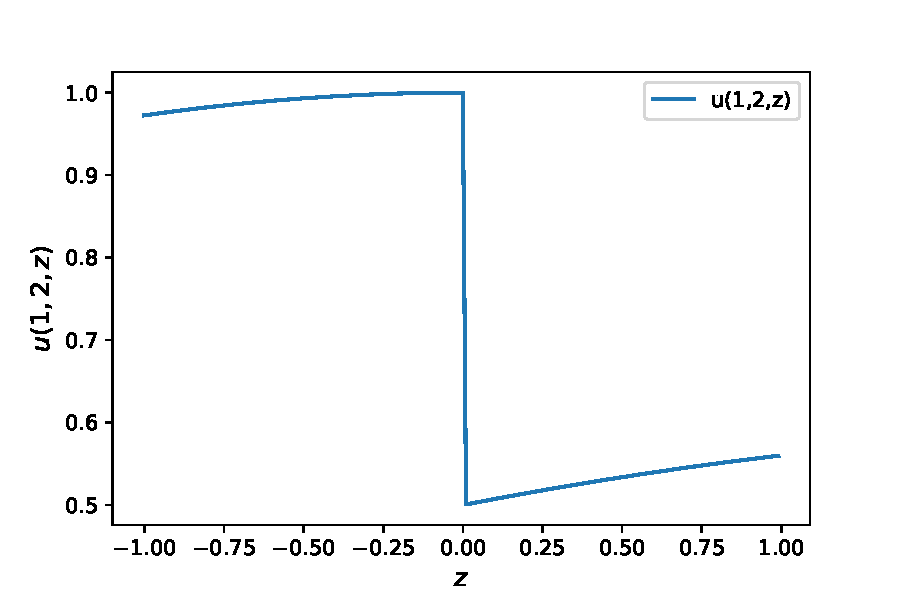
\includegraphics[width=0.8\textwidth]{gPC_hyp/c_discontinuous}
  \bicaption[2-1]{例一:显式解(\ref{ana_sol})在$t=1$和$x=2$处关于$z$间断。}{例一:显式解(\ref{ana_sol})在$t=1$和$x=2$处关于$z$间断。}{Fig}{Example 1. The analytic solution~(\ref{ana_sol}) at $t=1$ and $x=2$ is a discontinuous function of $z$.}
\end{figure}
% Figure\ref{1} shows that the analytic solution(\ref{ana_sol}) has a discontinuity at $z = 0$ when $x = 2$.  Figure\ref{2} shows that the expectation and variance of the analytic solution. In this case, one can expect a low  convergence rate of the standard gPC-SG method. 
图\ref{2-1}显示当$x = 2$时,显式解(\ref{ana_sol})在$z = 0$处有间断。图\ref{2-2}画出了显式解的期望值和方差。 在这种情况下,可以预期标准gPC-SG方法的收敛很慢。 
\begin{figure}[htbp]
  \centering
  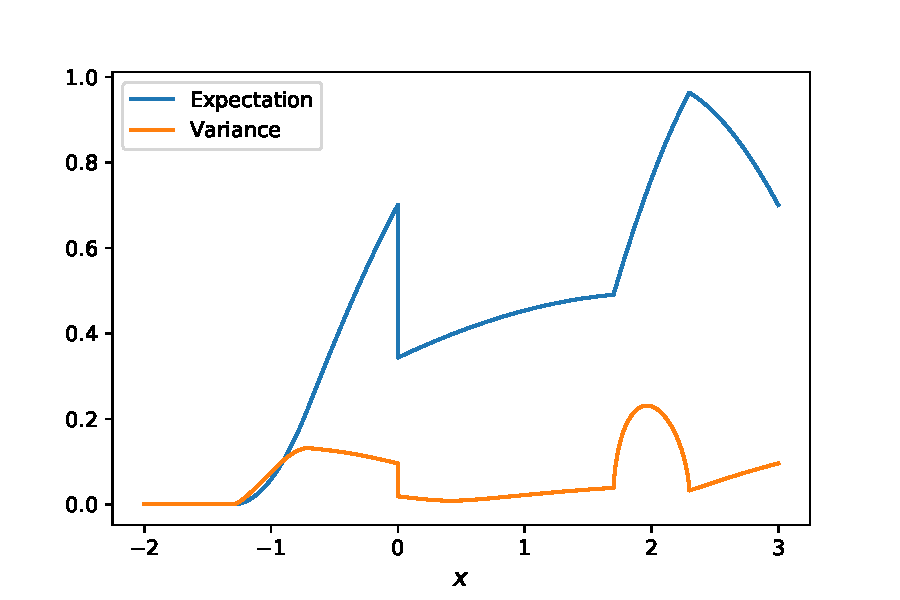
\includegraphics[width=0.8\textwidth]{gPC_hyp/c_exact}
  \bicaption[2-2]{例一:显式解的期望与方差。}{例一:显式解的期望与方差。}{Fig}{Example 1. The expectation and variance of the analytic solution.}
\end{figure}

\subsubsection{一阶差分逼近}
% In this subsection, we will give the numerical results of our discrete gPC-SG method.  Figure\ref{3} shows the numerical expectation and variance compared with the analytic solution with $\Dx = 0.001$, $\Dt = \dfrac{1}{4}\Dx$ and gPC order $K=20$. The discrepancy on the variance is due to the poor resolution of the
% first order spatial discretization, which is improved with the second order
% spatial discretization to be used later.
在本小节中,我们将给出离散gPC-SG方法的数值结果。图\ref{2-3}显示使用$\Dx = 0.001$,$\Dt = \dfrac{1}{4}\Dx$,gPC-SG阶数$K = 20$的数值解与显式解的期望与方差的比较。方差的误差是由一阶空间离散的低分辨率导致的。后面我们将使用二阶离散格式对其进行改进。

% Next we conduct the convergence test only for the gPC approximation.
% We fix $\Dx=0.005$ and $\Dt = \dfrac{1}{5}\Dx$ in all computations with
% different $K$. Figure\ref{4} shows that the $\ell^1$ error decays very fast with respect to the gPC order $K$. When $K=4$, it decays to the numerical error of the finite difference method. 
接下来,我们对gPC-SG进行收敛性测试。我们在所有计算中固定$\Dx=0.005$和$\Dt = \dfrac{1}{5}\Dx$。图\ref{2-4}显示$\ell^1$误差相对于gPC阶数$K$衰减得非常快。当$K=4$时,基本衰减到有限差分法的误差。
\begin{figure}[htbp]
  \includegraphics[width=0.5\textwidth]{gPC_hyp/c_mean}
  \includegraphics[width=0.5\textwidth]{gPC_hyp/c_var}
  \bicaption[2-3]{例一:一阶格式的数值解与显示解比较,$\Dx = 0.001$,$\Dt = \dfrac{1}{4}\Delta x$,gPC阶数$K=20$。}{例一:一阶格式的数值解与显示解比较,$\Dx = 0.001$,$\Dt = \dfrac{1}{4}\Delta x$,gPC阶数$K=20$。}{Fig}{Example 1. The analytic solution compared with the new gPC-SG method using first order finite difference approximation with $\Dx = 0.001$, $\Dt = \dfrac{1}{4}\Delta x$, gPC order $K=20$.}
\end{figure}


\begin{figure}[htbp]
  \centering
  \includegraphics[width=0.8\textwidth]{gPC_hyp/c_gpc_error}
  \bicaption[2-4]{例一:一阶离散格式$\ell^1$误差与gPC阶数的关系,$\Dx=0.005$, $\Dt=\dfrac{1}{5}\Dx$。}{例一:一阶离散格式$\ell^1$误差与gPC阶数的关系,$\Dx=0.005$, $\Dt=\dfrac{1}{5}\Dx$。}{Fig}{Example 1. The first order finite difference approximation with $\Dx=0.005$, $\Dt=\dfrac{1}{5}\Dx$: the $\ell^1$ error versus the gPC order.}
\end{figure}

% However, in Figure\ref{4}, since the finite difference error dominates the
% gPC error, it is difficult to verify the convergence rate of the gPC method. In order to examine the gPC error, we fix $\Dx$ and $\Dt$, and
% compare the numerical solutions with different $K$, with the case of $K=30$ serving as the reference solution.  We measure the $\ell^1$ error between each $K=2,3,\dotsc,20$ and $K=30$. The result is shown 
% in Figure\ref{5}, in which an exponential convergence in the gPC approximation can be observed by using the $\log$-$\log$ plot. Note that if the convergence order is algebraic, the curve should be a line.
% Here the curve shape shows the  exponential decay of the gPC error.

然而,在图\ref{2-4}中,由于有限差分的误差占主导地位(远大于gPC-SG方法的误差),这样很难验证gPC方法的收敛速度。为了验证gPC-SG的收敛性,我们固定$\Dx$和$\Dt$,用作为$K = 30$时的解作为参考解,比较$K$不同时与参考解的差别。 我们测量每个$K=2,3,\dotsc,20$和$K =30$之间的$\ell^1$误差,结果如图\ref{2-5}所示。通过对数图可以观察到gPC-SG方法是指数收敛的。

\begin{figure}[htbp]
  \centering
  \includegraphics[width=0.8\textwidth]{gPC_hyp/c_gpc_error_loglog}
  %\includegraphics[width=0.5\textwidth]{figs/c_gpc_error_logy}
  \bicaption[2-5]{例一:一阶格式的gPC-SG方法误差与gPC阶数的对数关系,$\Dx=0.005$, $\Dt=\dfrac{1}{5}\Dx$。}{例一:一阶格式的gPC-SG方法误差与gPC阶数的对数关系,$\Dx=0.005$, $\Dt=\dfrac{1}{5}\Dx$。}{Fig}{Example 1. The first order finite difference approximation $\Dx=0.005$, $\Dt=\dfrac{1}{5}\Dx$: the gPC error versus the gPC order by a log-log plot
(with other numerical parameters fixed).}
\end{figure}


%
%\begin{equation}
%  \begin{split}
%    &\text{error} \sim \mathrm{e}^{-N} \\
%    \Leftrightarrow&\log(\text{error}) \sim -N \\
%    \Leftrightarrow&\log(\text{error}) \sim -\mathrm{e}^{\log(N)}.
%  \end{split}
%\end{equation}


\subsubsection{二阶差分逼近}
% For the second order scheme, we use the same set up as in the first order case. Figure\ref{mv2} shows the expectation and variance compared with the analytic solution,
% which gives a more accurate solution than the first
% order approximation especially for the variance around $x=2$. 

% Figure\ref{mverr2} and Figure\ref{mverrlog2} show the convergence of the numerical method in the gPC order from which one can observe the fast convergence. Comparing Figure 7 with Figure 4, we can see that the second scheme has a better total $\ell^1$ error. But the rate of the gPC convergence shown in Figure\ref{mverrlog2} is  not as fast as the first order scheme. This is hardly surprising since our spectral convergence
% depends on the smoothness of the discrete solutions, and the smoothness is
% given by the numerical viscosity which is larger 
% for the first order spatial discretization. The second order spatial
% discretization offers better accuracy away from the discontinuities and better
% resolutions at discontinuities, but  because it is closer
% to the analytic solution (which is not smooth) thus less smooth than the first order one, and smoothness of the discrete solution is what 
%  our spectral convergence relies upon, thus its gPC congerence rate, compared with
% the first order one, should be slower.  However this does not mean that 
% the second order method is inferior to the first one, since one has to 
% consider the {\it overall} error, including the contributions of error from
% the spatial discretization in this problem. By comparing  Figure 6 with Figure 3, and 
% Figure 7 with Figure 4, it is obvious that the second order scheme outperforms
% the first order one.

对于二阶格式,我们用与前面一阶格式相同的设置。图\ref{mv2}画出了与显示解相比的期望值和方差,可以看到比一阶格式的结果要好,特别是方差在$x = 2$附近的近似。

图\ref{mverr2}和图\ref{mverrlog2}显示了gPC-SG方法的收敛,从中可以观察到收敛是非常之快的。比较图\ref{mverr2}和图\ref{2-4},我们可以看到二阶格式有更好的总$\ell^1$误差。但是图\ref{mverrlog2}中显示的gPC收敛的速率却不如一节格式。这点并不奇怪,因为我们的收敛速率取决于离散解的光滑性,而一阶格式给出的数值粘性较大,从而光滑性更好。二阶格式因为它更接近
于精确解(其是非常不光滑的),因此与一阶格式相比离散解的光滑性相对比较差,而这正是影响收敛速率的主要因素,所以二阶格式的收敛速度相比一阶而言较慢。然而这并不意味着二阶格式不如一阶,因为必须考虑{\it 整体的}误差,包括空间离散的误差。通过比较图\ref{mv2}与图\ref{2-3},图\ref{mverr2}与图\ref{2-4},显然二阶格式要优于一阶格式。
 
% RecaThis is due to the different treatments we use for gPC-SG method: in the f%irst order scheme we use the standard gPC-SG procedure, \ie, we can compute the% gPC projection matrix analytically, however, in the second order case we use n%umerical integration to compute the projection matrix due to the nonlinearity. %The error of numerical integration affects the convergence here which is shown %clearly between Figure 8 and Figure 5: the gPC error for the second order schem%e is larger than that for the first order scheme, \ie, when gPC $K=20$ error of% second order scheme $O(10^{-4})$ versus $O(10^{-15})$ for the first order sche%me.  
\begin{figure}[htbp]
  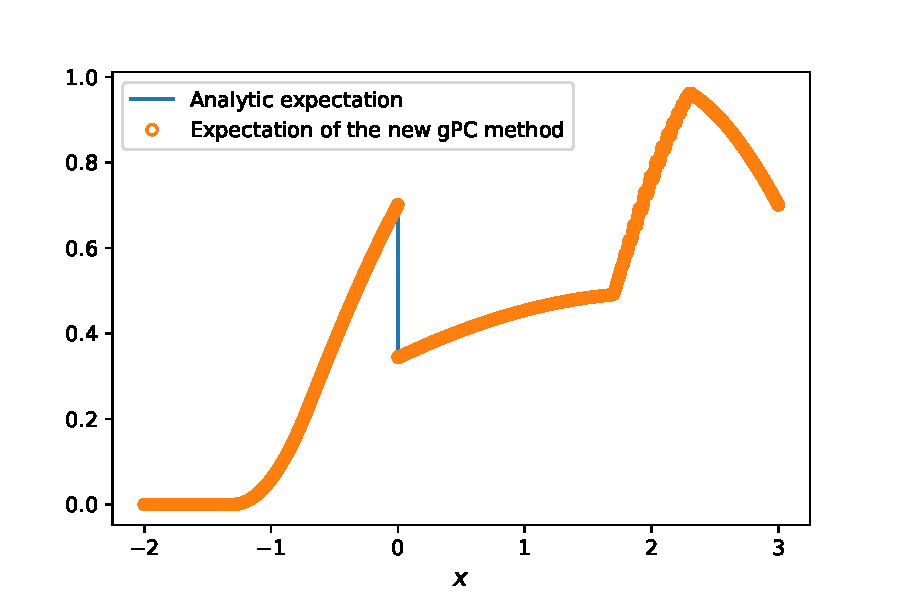
\includegraphics[width=0.5\textwidth]{gPC_hyp/mean2}
  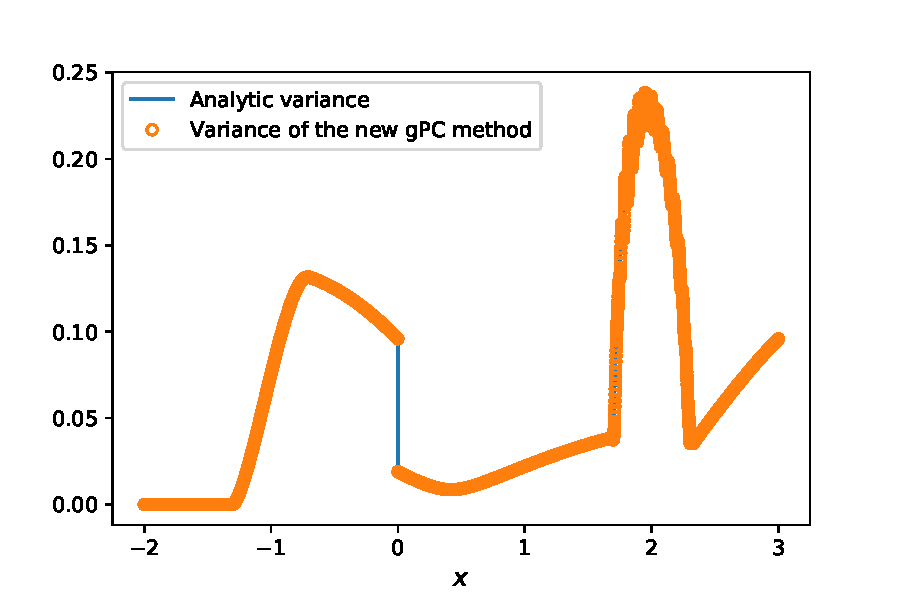
\includegraphics[width=0.5\textwidth]{gPC_hyp/var2}
  \bicaption[mv2]{例一:显式解与二阶空间离散的gPC-SG方法比较,$\Delta x = 0.001$, $\Delta t = \dfrac{1}{4}\Delta x$,gPC-SG的阶数为$K=20$。}{例一:显式解与二阶空间离散的gPC-SG方法比较,$\Delta x = 0.001$, $\Delta t = \dfrac{1}{4}\Delta x$,gPC-SG的阶数为$K=20$。}{Fig}{Example 1. The analytic solution compared with the new gPC-SG method using the second order finite difference approximation with  $\Delta x = 0.001$, $\Delta t = \dfrac{1}{4}\Delta x$, gPC order $K=20$.}
\end{figure}

\begin{figure}[htbp]
  \centering
  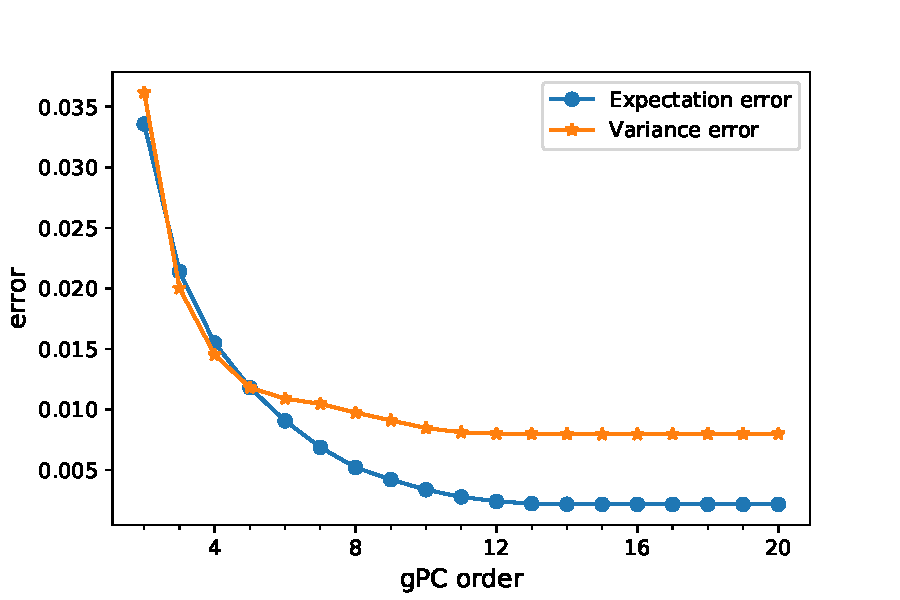
\includegraphics[width=0.8\textwidth]{gPC_hyp/gpc_err2}
  \bicaption[mverr2]{例一:二阶格式$\ell^1$误差与gPC阶数的关系,$\Dx=0.005$,$\Dt=\dfrac{1}{5}\Dx$。}{例一:二阶格式$\ell^1$误差与gPC阶数的关系,$\Dx=0.005$,$\Dt=\dfrac{1}{5}\Dx$。}{Fig}{Example 1. The second order finite difference approximation $\Dx=0.005$, $\Dt=\dfrac{1}{5}\Dx$: the 
  $\ell^1$ error versus the gPC order.}
\end{figure}

\begin{figure}[htbp]
  \centering
  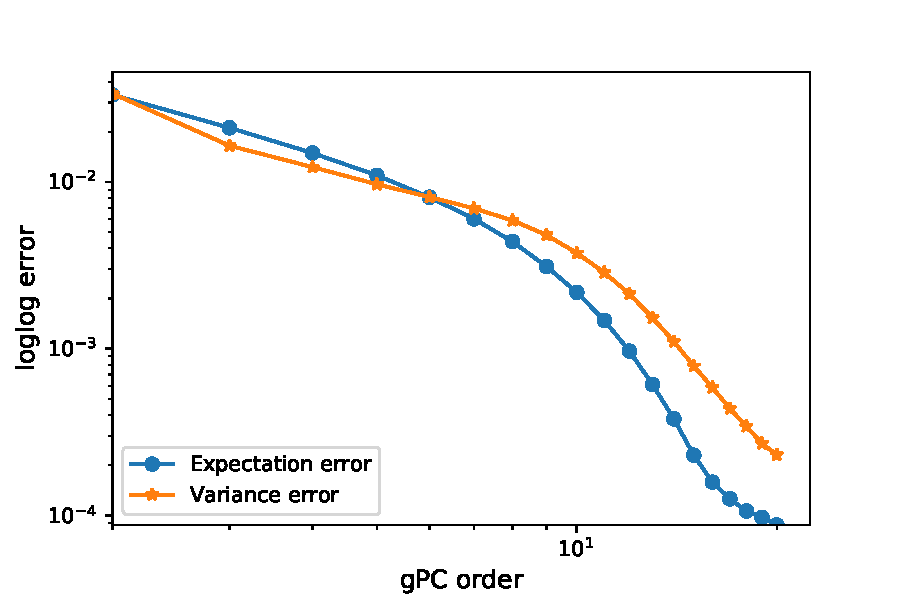
\includegraphics[width=0.8\textwidth]{gPC_hyp/gpc_err2_loglog}
  %\includegraphics[width=0.5\textwidth]{figs/gpc_err2_logy}
  \bicaption[mverrlog2]{例一:二阶格式$\ell^1$误差与gPC阶数的对数关系,$\Dx=0.005$,$\Dt=\dfrac{1}{5}\Dx$。}{例一:二阶格式$\ell^1$误差与gPC阶数的对数关系,$\Dx=0.005$,$\Dt=\dfrac{1}{5}\Dx$。}{Fig}{Example 1. The second order finite difference approximation $\Dx=0.005$, $\Dt=\dfrac{1}{5}\Dx$: the gPC error versus the gPC order by a log-log plot (with other numerical parameters fixed).}
  % \label{mverrlog2}
\end{figure}

%From numerical analysis point of view, you want to estimate the error between final numerical solution $\mathbf{U}^N_{h}$ and the exact solution $u$ on some norm, you can do this in two different ways:
%\begin{equation} \label{error1}
%||\mathbf{U}^N_{h}-u||\leq||\mathbf{U}^N_{h}-\mathbf{U}^N||+||\mathbf{U}^N-u||
%\end{equation}
%or
%\begin{equation} \label{error2}
% ||\mathbf{U}^N_{h}-u||\leq||\mathbf{U}^N_{h}-U_h||+||U_h-u||.
%\end{equation}
%And for our problem if you do as (\ref{error1}), the $||\mathbf{U}^N-u||$ part can not be estimated. If you do in the second way (\ref{error2}), $|U_h-u||$ can be obtained as the same in Qi Peng's paper (that depends on $z$), $||\mathbf{U}^N_{h}-U_h||$ can be obtained in the standard gPC way. 

\subsection{例二:带有随机间断势的刘维尔方程}

再次写出刘维尔方程
\begin{equation}
  u_t+v u_x-V_x u_v=0, \quad t>0, \quad x,v\in R,
\end{equation}
其中随机势如下
\begin{equation}
  V(x,y)=V_0(x)+0.1xz,
\end{equation}
$z$为$(-1,1)$上的均匀分布,
\begin{equation}
  V_0(x)=
  \begin{cases}
    0.2, \quad &x<0, \\
    0, \quad &x>0.
  \end{cases}
\end{equation}

% For the given initial data, one cannot get an analytic solution for this problem. Instead we will use the {\it collocation method} as a comparison. In collocation method, one solves the Liouville equation(\ref{eq_Liou}) at a discrete set of $\{z_i\}_{1\leq i\leq M}$ called sample points in the corresponding random space. For every fixed $z_i$, we only need to solve a {\it deterministic} Liouville equation with discontinuous potential using Hamilton preserving scheme\citen{Wen:2005ueba}. Then the expectation and variance can be obtained by the quadrature rules of(\ref{exp}) and(\ref{var}). In the following examples, we choose $\{z_i\}_{1\leq i\leq M}$ as the roots of $M$th order Legendre polynomials and use the Gauss-Legendre quadrature to obtain the expectation and variance.

对于给定的初始数据,因为无法得到这个问题的显式精确解。所以,我们将使用{\it 配点法}(stochastic collocation method)作为参考解。在配点法中,在对应的随机空间中取$\{z_i\}_{1\leq i\leq M}$的离散点集合,称为抽样点,我们在只需在抽样点上解刘维尔方程(\ref{eq_Liou})。 对于每个固定的$z_i$,我们只需要使用用来解{\it 确定性} 的带间断势的刘维尔方程的哈密顿守恒格式。然后,可以通过(\ref{exp})和(\ref{var})通过数值积分获得期望和方差。在以下示例中,我们选择$\{z_i\}_{1\leq i\leq M}$作为$M$阶勒让德多项式的根,并使用高斯积分来获得期望值和方差。

% For the gPC method we need to evaluate $\int_{-1}^1 V_0(z)P_j(z)P_k(z) \rho(z)\diff z$, which, for this simple case, is given by
对于gPC-SG方法我们需要计算$\int_{-1}^1 V_0(z)P_j(z)P_k(z) \rho(z)\diff z$也就是,
\begin{equation}
  \int_{-1}^1 V_0(z)P_j(z)P_k(z) \rho(z)\diff z =
  \begin{cases}
    \dfrac{j+1}{\sqrt{(2j+1)(2j+3)}}, &k=j+1, \\
    V'_0(x), &k=j, \\
    \dfrac{j}{\sqrt{4j^2-1}}, &k=j-1.
  \end{cases}
\end{equation}
这里我们得到一个对称的三对角矩阵。

% As an illustration of the singularity of the solution caused by the discontinuous potential , we use a continuous initial data:
为了说明由间断的势导致的解的奇异性,我们使用连续的初值:
\begin{equation}
  u(x,v,0)=
  \begin{cases}
  \sin[2\pi(0.25-(x^2+v^2))], &x^2+v^2<0.25, \\
  0, &\text{其他}.
  \end{cases}
\label{ex2-init2}
\end{equation}
% The expectation of the solution by using the collocation method with $M=20$ sample points and our new gPC-SG method with gPC order $K=4$ are shown in Figure\ref{2-8}. 
由配点法($M=20$个抽样点)和我们的$K=4$阶离散gPC-SG方法期望与方差如下图\ref{2-8}所示。
\begin{figure}[htbp]
  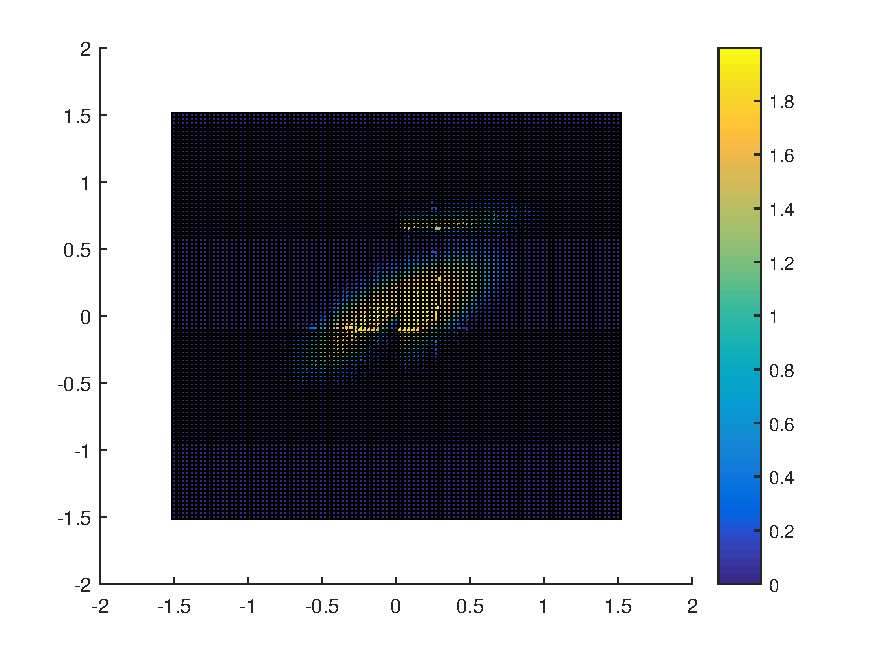
\includegraphics[width=0.5\textwidth]{gPC_hyp/pseudoSpecSmooth}
  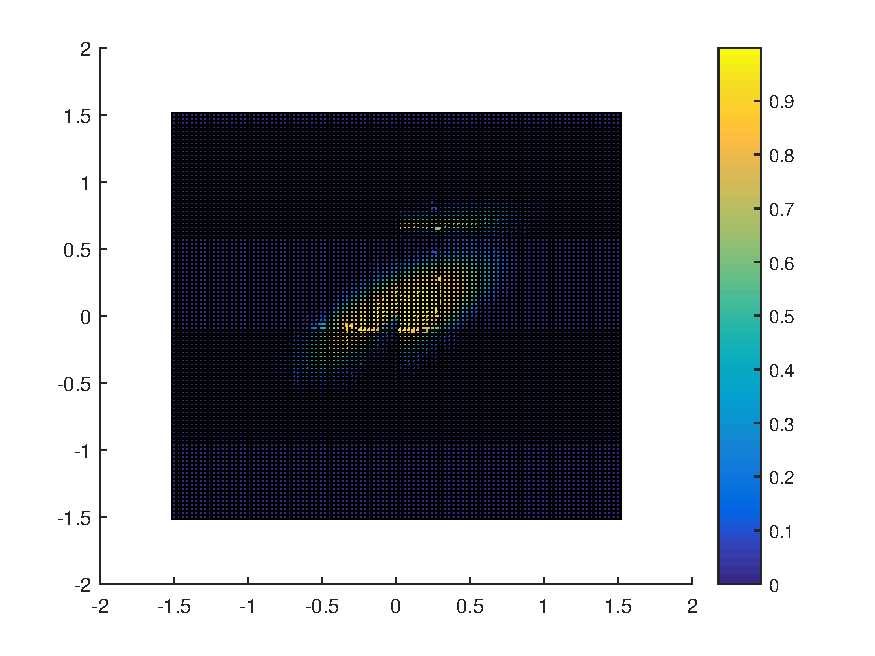
\includegraphics[width=0.5\textwidth]{gPC_hyp/galerkinsmooth}
  \bicaption[2-8]{例二:初值为(\ref{ex2-init2})。由配点法(左)与离散gPC-SG方法(右)得到的期望。}{例二:初值为(\ref{ex2-init2})。由配点法(左)与离散gPC-SG方法(右)得到的期望。}{Fig}{Example 2 with initial data (\ref{ex2-init2}). Expectation of the solution. Left: the collocation method with $20$ sample points. Right: the new gPC-SG method with gPC order $K=4$.}
  % \label{2-8}
\end{figure}
% Although the initial data is continuous, due to the interface condition, the solution may still be discontinuous. This singularity will have a big impact on the convergence of gPC method.
虽然初值是连续的,但由于界面条件的存在,解仍然是间断的。而这种奇异性会大大影响gPC-SG方法的收敛性。

\subsubsection{一阶差分逼近}
在这个例子里,我们考虑初值
\begin{equation}
  u(x,v,0)=
  \begin{cases}
    1, \quad &x\geq 0, v<0, x^2+v^2<1, \\
    1, \quad &x\leq 0, v>0, x^2+v^2<1, \\
    0, \quad &\text{其他}.
  \end{cases}
\label{ex2-init1}
\end{equation}
% Notice that the solution has singularity due to both the initial data and the discontinuous potential. The deterministic version of this example was used in\citen{Wen:2005ueba} and the analytic solution can be obtained by using the method of characteristics. We first plot the analytic solution and numerical solution (using the first order flux) with a fixed $z=0$ in Figure\ref{2-9} corresponding to the deterministic example in\citen{Wen:2005ueba}.

注意,由于初始数据和势的不连续性从而导致解具有奇异性。该示例的确定性版本在\citen{Wen:2005ueba}中被使用过,并且可以通过使用特征线的方法获得显式精确解。 我们首先在画出对应于\citen{Wen:2005ueba}中的确定性示例的图\ref{2-9},包括显示精确解和数值解(使用一阶通量),其中固定$z = 0$。
\begin{figure}
  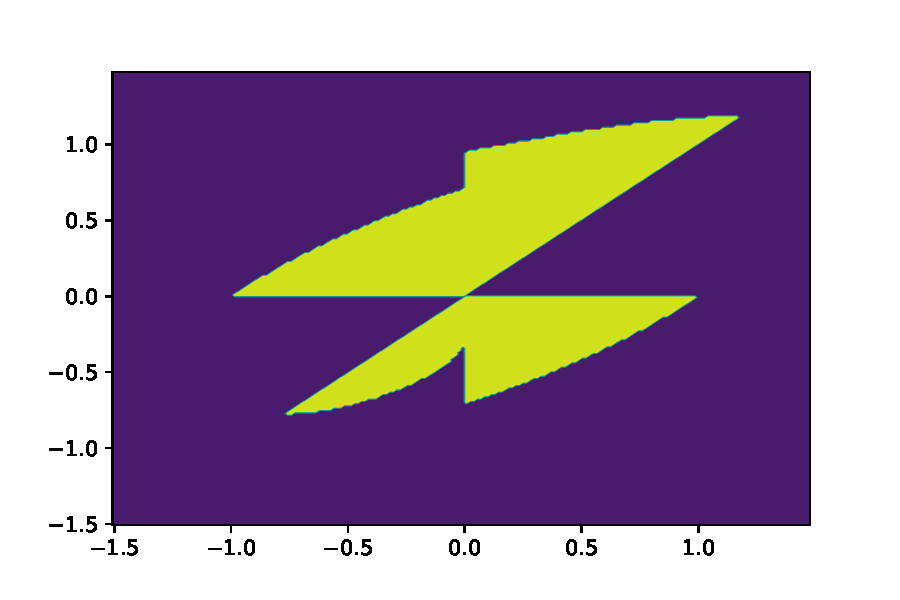
\includegraphics[width=0.5\textwidth]{gPC_hyp/exact}
  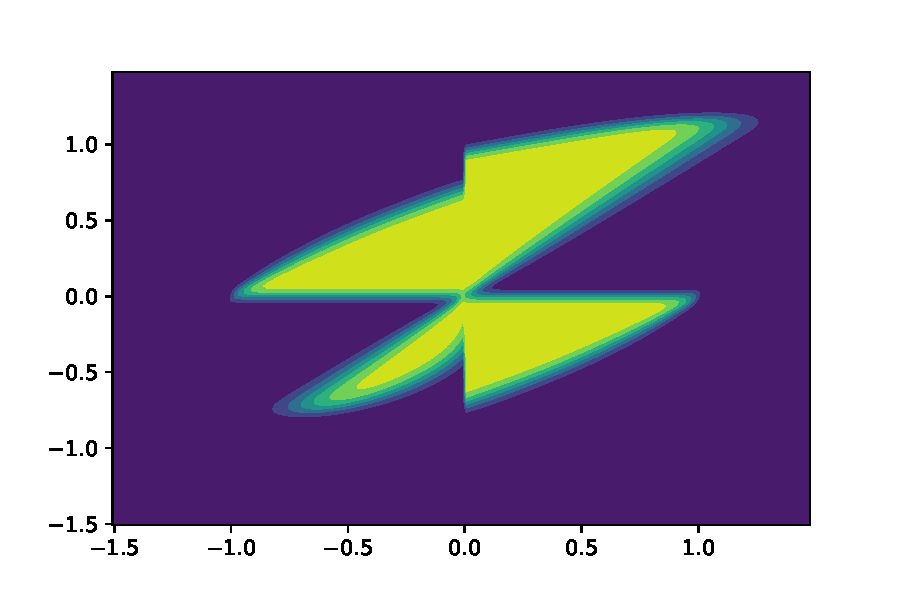
\includegraphics[width=0.5\textwidth]{gPC_hyp/num_1}
  \bicaption[2-9]{例二的确定性版本,初值(\ref{ex2-init1})。显式精确解(左),数值解(右),$\Delta x = \Delta v = 0.015$,$\Delta t = 0.001$。}{例二的确定性版本,初值(\ref{ex2-init1})。显式精确解(左),数值解(右),$\Delta x = \Delta v = 0.015$,$\Delta t = 0.001$。}{Fig}{The deterministic case of Example 2 with initial data (\ref{ex2-init1}). Left: analytic solution of the deterministic problem with $z=0$ and $t=1$. Right: numerical solution using the first order Hamiltonian preserving scheme with $\Delta x = \Delta v = 0.015$, $\Delta t = 0.001$.}
  % \label{2-9}
\end{figure}

% Then we compare the solution computed by the collocation method with $M=20$ sample points (Figures\ref{2-6} and\ref{2-15} left). Figures\ref{2-6} and\ref{2-15} right show the solutions  by our new gPC-SG method with gPC order $K=10$. Here the mesh size is $\Dx=\Dv=0.03$ and time step is $\Dt=0.002$. One can see the difference between the expectation of the stochastic solution and the deterministic case when $z=0$ and this differences can be easily seen on the variance plots as well. The expectation of the stochastic solution is expected to be smoother
% since it integrates over the $z$ variable, thus gains on order of regularity
% (see examples in \citen{Des, HJX}).
% For the computation cost, our new gPC-SG method runs much faster than collocation method. The collocation method takes about $20$ times cost of the deterministic version due to $20$ sample points we choose, however, our new gPC-SG,
% with $K=10$,  takes about $10$ times the cost of the deterministic problem.

然后我们与用配点法计算的解($M = 20$样本点)(图\ref{2-6}和\ref{2-15}左)进行比较。图\ref{2-6}和\ref{2-15}右显示我们的新gPC-SG方法的解,其中gPC阶数$K = 10$。这里的网格大小是$\Dx = \Dv = 0.03$,时间步长是$\Dt = 0.002$。可以看到随机方程的解的期望和当$z = 0$的确定性情况之间的差异,并且这种差异也可以容易地在方差图上看出。随机方程的解的期望更加光滑,因为它对$z$变量进行了积分(相当于平均),从而得到了更好的正则性(参见\citen{Des, HJX})。关于计算的开销,我们的新的离散gPC-SG方法运行比配点法要快得多。 配点法要花费大约$20$倍确定性版本的成本,因为我们使用了$20$个样本点;然而,我们的新的离散gPC-SG,阶数$K = 10$(即可得到优于配点法$20$个样本点的解),花费大约$10$倍确定性问题的成本。

\begin{figure}[htbp]
% \centering
  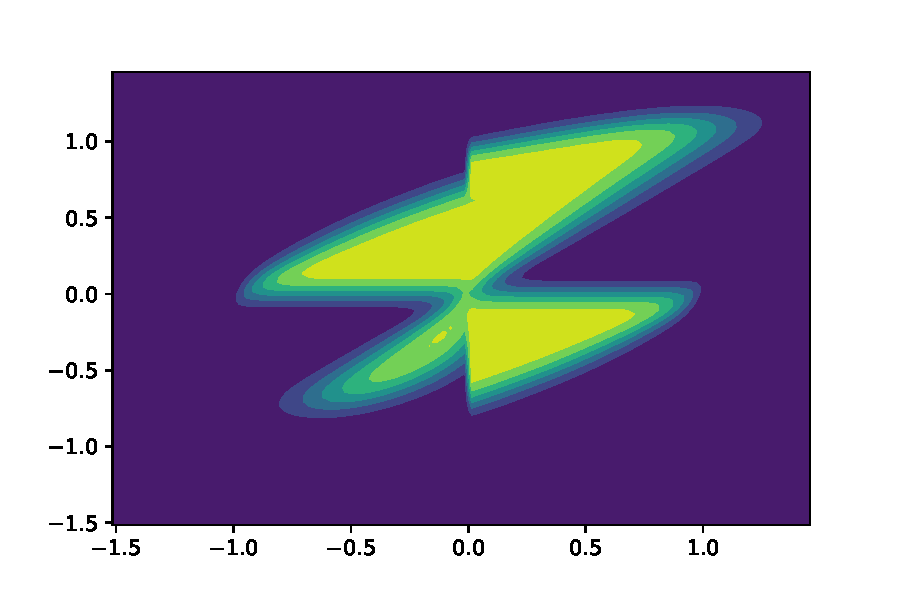
\includegraphics[width=0.5\textwidth]{gPC_hyp/col_mean_1}
  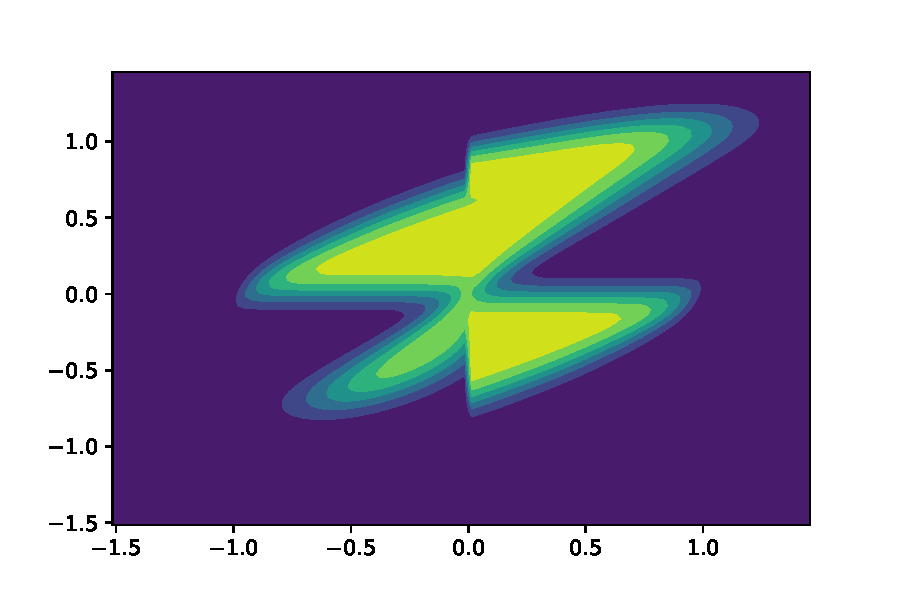
\includegraphics[width=0.5\textwidth]{gPC_hyp/mean_1}
  \bicaption[2-6]{例二:初值为(\ref{ex2-init1}),由一阶差分格式得到的期望,配点法(左)与离散gPC-SG方法(右),$\Dx=\Dv=0.03$,$\Dt=0.002$。}{例二:初值为(\ref{ex2-init1}),由一阶差分格式得到的期望,配点法(左)与离散gPC-SG方法(右),$\Dx=\Dv=0.03$,$\Dt=0.002$。}{Fig}{Example 2 with initial data (\ref{ex2-init1})  by the first order 
finite difference approximation  with $\Dx=\Dv=0.03$ and $\Dt=0.002$.  The expectation of the solution. Left: the collocation method with $M=20$ samples points. Right: the new gPC-SG method using first order finite difference approximation.}
  % \label{2-6}
\end{figure}
\begin{figure}[htbp]
% \centering
  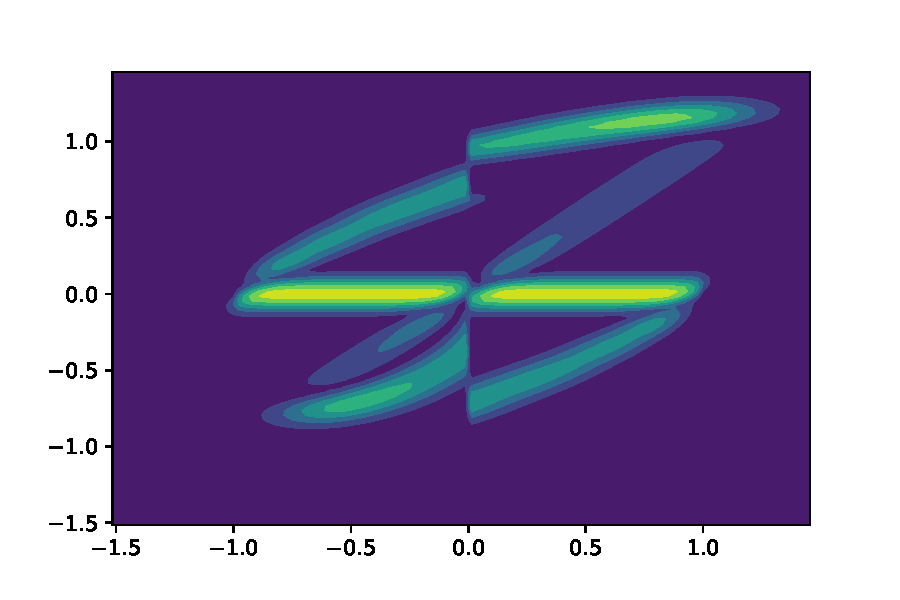
\includegraphics[width=0.5\textwidth]{gPC_hyp/col_var_1}
  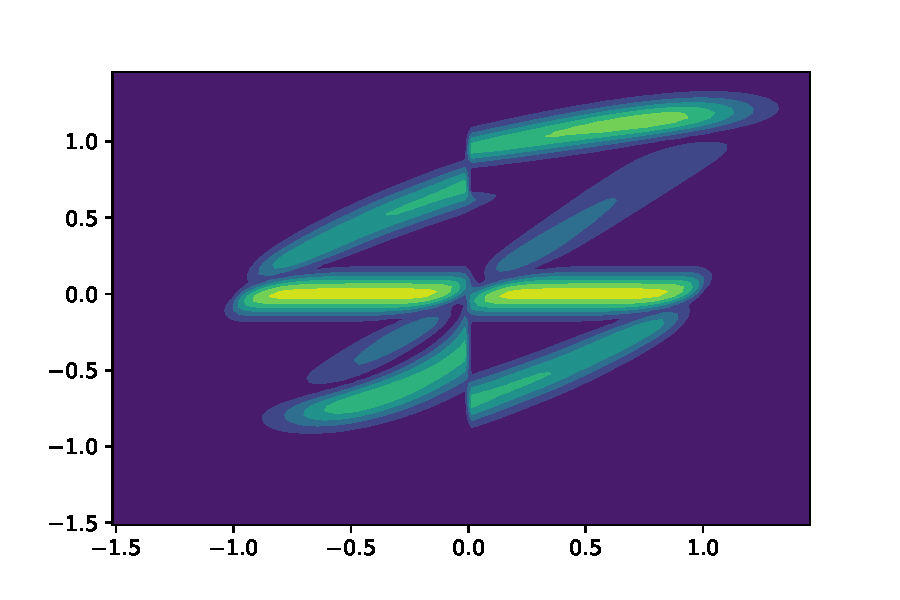
\includegraphics[width=0.5\textwidth]{gPC_hyp/var_1}
  \bicaption[2-15]{例二:初值为(\ref{ex2-init1}),由一阶差分格式得到的方差,配点法(左)与离散gPC-SG方法(右),$\Dx=\Dv=0.03$,$\Dt=0.002$。}{例二:初值为(\ref{ex2-init1}),由一阶差分格式得到的方差,配点法(左)与离散gPC-SG方法(右),$\Dx=\Dv=0.03$,$\Dt=0.002$。}{Fig}{Example 2 with initial data (\ref{ex2-init1}) by the first order 
finite difference approximation  with $\Dx=\Dv=0.03$ and $\Dt=0.002$. The variance of the solution. Left: the collocation method. Right: the new gPC-SG 
method.}
  % \label{2-15}
\end{figure} 

% In Figure\ref{2-7} we plot the $\ell^1$ error of the discrete gPC-SG method as the gPC order $K$ increases. This figure shows the spectral convergence.
在图\ref{2-7},我们画出离散gPC-SG方法的$\ell^1$误差随着gPC阶数$K$增加的变化关系,显示出了谱收敛结果。
\begin{figure}[htbp]
  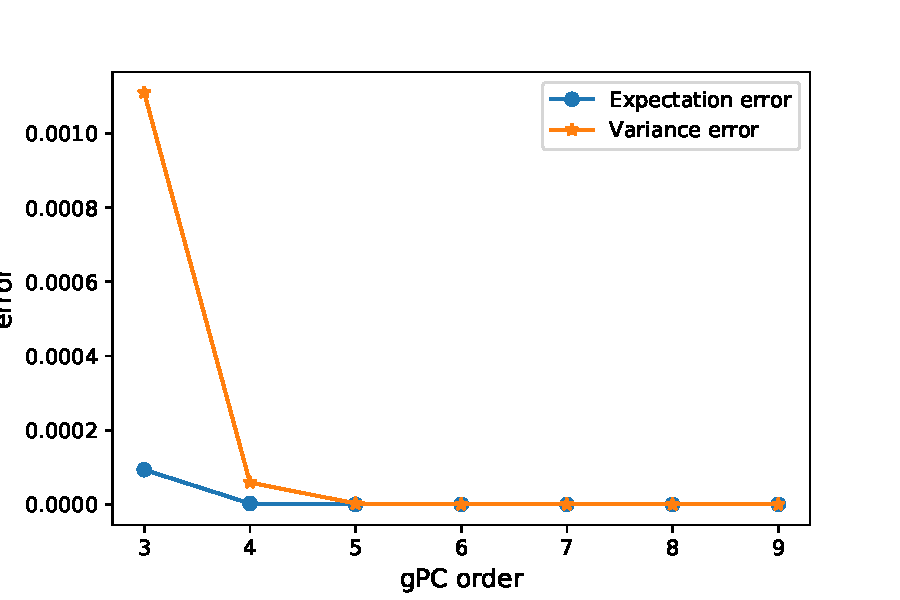
\includegraphics[width=0.5\textwidth]{gPC_hyp/convergence_1}
  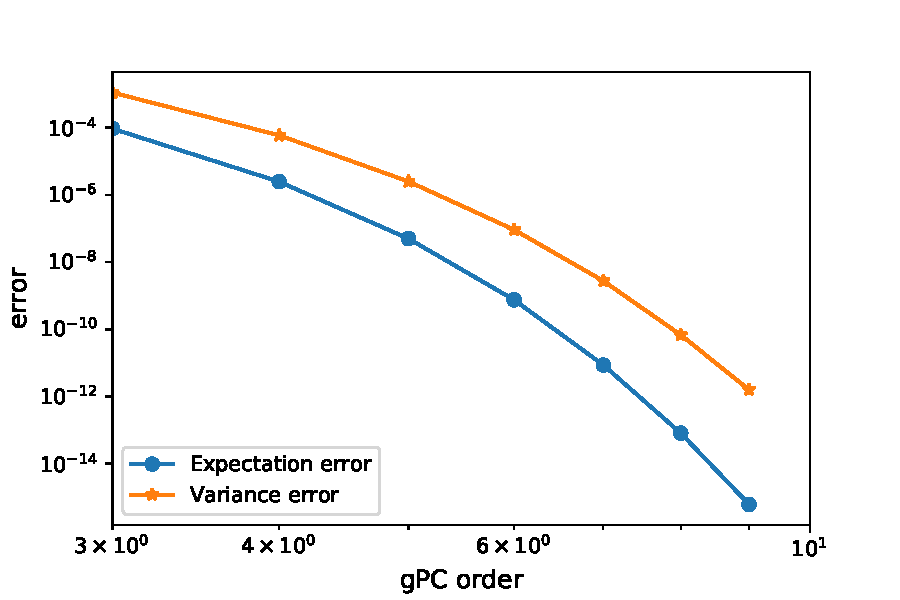
\includegraphics[width=0.5\textwidth]{gPC_hyp/loglog_conv_1}
  \bicaption[2-7]{例二:初值(\ref{ex2-init1}),一阶离散gPC-SG方法的$\ell^1$误差随着gPC阶数$K$增加的变化关系(左)及对数图(右)。}{例二:初值(\ref{ex2-init1}),一阶离散gPC-SG方法的$\ell^1$误差随着gPC阶数$K$增加的变化关系(左)及对数图(右)。}{Fig}{Example 2 with initial data (\ref{ex2-init1}). Convergence of the new gPC-SG method using the first order finite difference approximation. Left: the $\ell^1$ error versus gPC order. Right: the gPC error versus the gPC order by a log-log plot (with other numerical parameters fixed).}
  % \label{2-7}
\end{figure}






\subsubsection{二阶差分格式}
% Here for the second finite difference approximation we still use the same set up as in previous subsection for the first order case. 
这里对于二阶差分格式,我们使用和前面一阶格式类似的参数设定。
% We also calculate the $\ell^1$ error between our numerical method ({\bf Jin remark: is this for deterministic or random potential?  If deterministic, what do you mean ``our method'' and why you need this which was already known previously?}) and the reference solution, and the results are given in Table\ref{10}.
% \begin{table}
% \centering
%   \begin{tabular}{ c|c|c|c| }
%   $\Delta x$ & 0.06 & 0.03 & 0.015 \\ \hline
%   $\ell^1$ error & 0.288 & 0.165 & 0.094 \\
% \end{tabular}
%   \caption{$\ell^1$ error and meshsize}
%   \label{10}
% \end{table}
% We can see that although we use a second order flux, the whole scheme's convergence rate cannot be more than half, as was previously proven
% in \citen{Wen:2005ueba,Qi:2013byba}.

% First as in the first order case, we will show the numerical solution of the deterministic case when $z=0$ using the second order flux in Figure\ref{deter_sec}.  The second order method clearly gives a much sharper resolution for the discontinuities than the first order method (compare the right figures of
% Figure 10 and Figure 15). But due to the Lax-Wendroff scheme we use in the $v$-direction(\ref{vflux}), there exists some oscillations due to numerical dispersion.
首先,如同一阶的情形,我们在\ref{deter_sec}中画出由二阶格式得到的$z=0$时确定性的方程的数值解。二阶格式明显给出了高分辨率的结果(相比一阶格式,见图\ref{2-9}和图\ref{2-11})。但是由于在$v$方向我们用的是Lax-Wendroff格式,所以这里有一些数值振荡。
\begin{figure}{}
  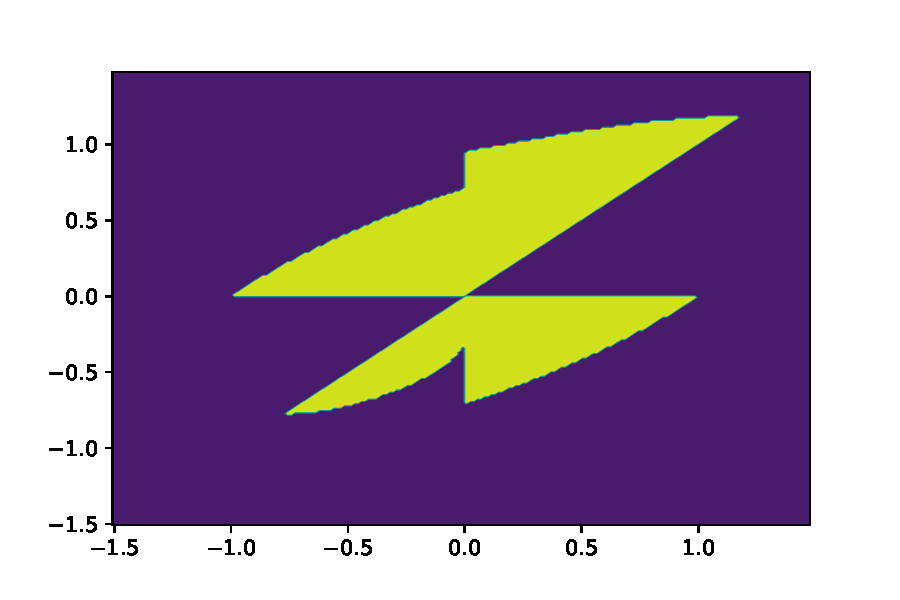
\includegraphics[width=0.5\textwidth]{gPC_hyp/exact}
  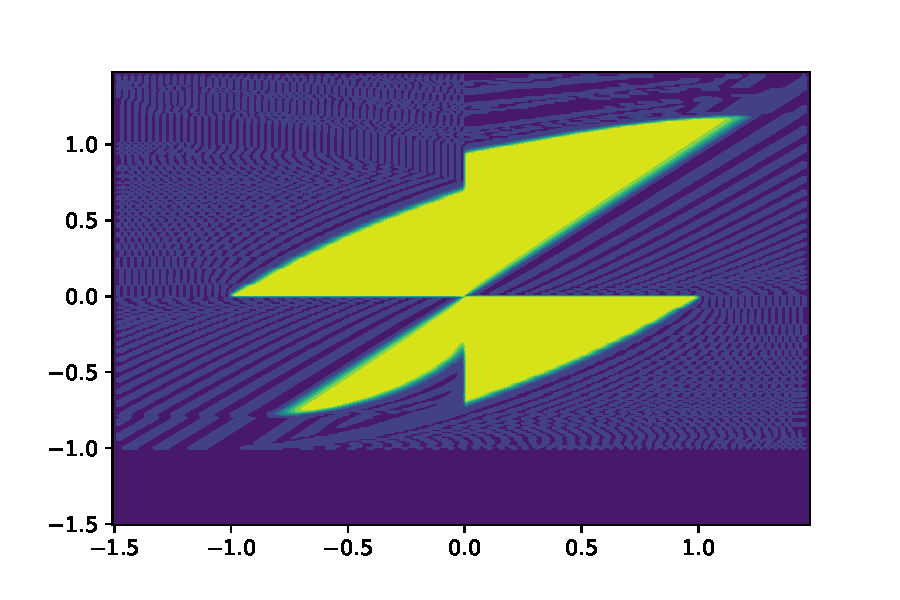
\includegraphics[width=0.5\textwidth]{gPC_hyp/num}
  \bicaption[deter_sec]{例二:初值为(\ref{ex2-init1})的确定性版本。左图为显式精确解($z=0$,$t=1$);右图为二阶格式的数值解,$\Delta x = \Delta v = 0.015$,$\Delta t = 0.001$。}{例二:初值为(\ref{ex2-init1})的确定性版本。左图为显式精确解($z=0$,$t=1$);右图为二阶格式的数值解,$\Delta x = \Delta v = 0.015$,$\Delta t = 0.001$。}{Fig}{The deterministic case of Example 2 with initial data~(\ref{ex2-init1}). Left: analytic solution of the deterministic problem with $z=0$ and $t=1$. Right: numerical solution using the second order Hamiltonian preserving scheme with $\Delta x = \Delta v = 0.015$, $\Delta t = 0.001$}
  % \label{deter_sec}
\end{figure}

% Then we will show the expectation and variance of the solution calculated by the collocation method with $M=20$ sample points and our new gPC-SG method (for the calculation of $\left<\mathrm{RHS}(z)\right>$ we also use 20 Gauss-Legendre quadrature points). See Figure\ref{2-11} and Figure\ref{2-12}.
接下来我们对比由配点法和离散gPC-SG方法计算的期望与方差,见图\ref{2-11}和\ref{2-12}:
\begin{figure}
  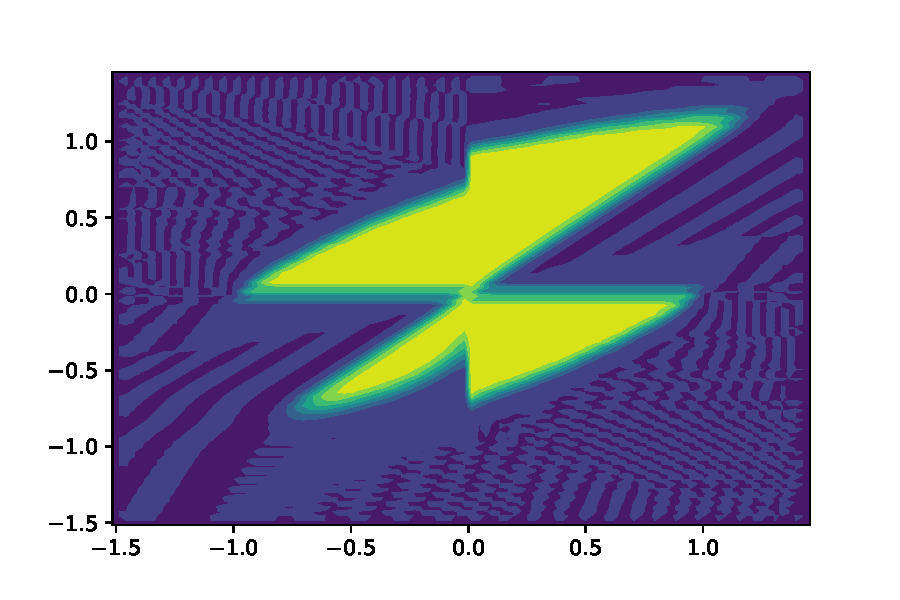
\includegraphics[width=0.5\textwidth]{gPC_hyp/col_mean}
  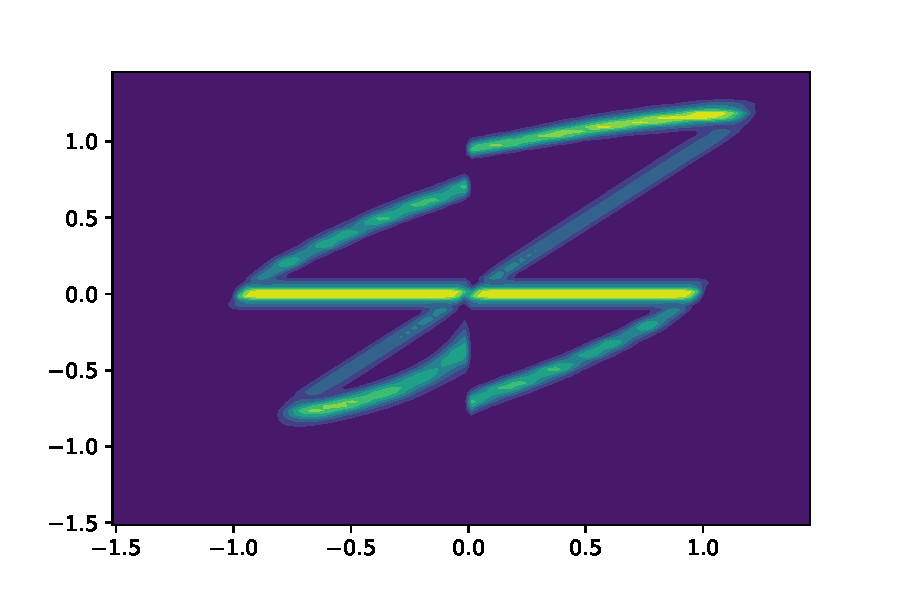
\includegraphics[width=0.5\textwidth]{gPC_hyp/col_var}
  \bicaption[2-11]{例二:初值为\ref{ex2-init1}),二阶离散配点法的解,期望(左)和方差(右),$\Delta x = \Delta v = 0.03$,$\Delta t = 0.002$。}{例二:初值为\ref{ex2-init1}),二阶离散配点法的解,期望(左)和方差(右),$\Delta x = \Delta v = 0.03$,$\Delta t = 0.002$。}{Fig}{Example 2 with initial data (\ref{ex2-init1}) by the second order 
finite difference approximation  with $\Delta x = \Delta v = 0.03$, $\Delta t = 0.002$. Reference solution 
 by the collocation method with 20 sample points at $t=1$. Left: expectation. Right: variance.}
  % \label{2-11}
\end{figure}
\begin{figure}
  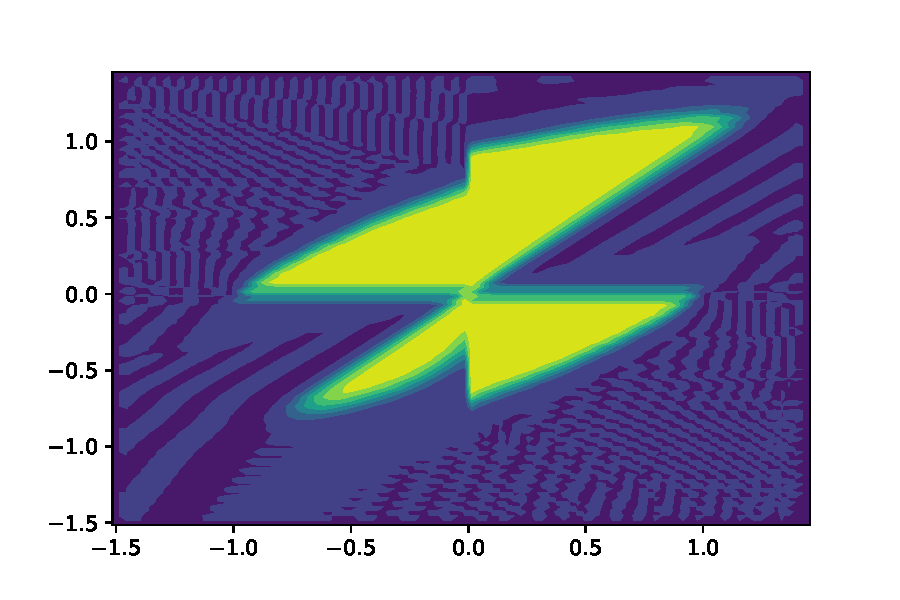
\includegraphics[width=0.5\textwidth]{gPC_hyp/mean}
  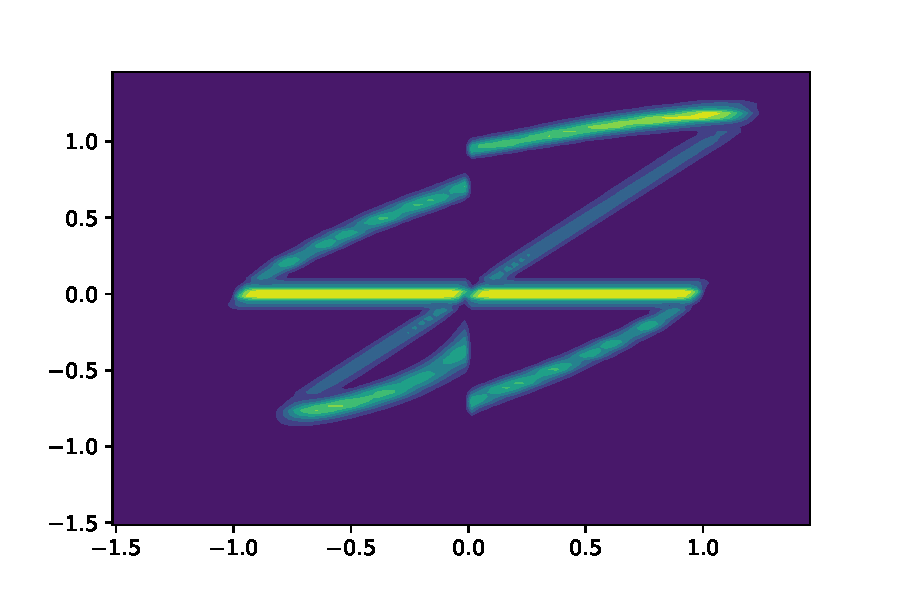
\includegraphics[width=0.5\textwidth]{gPC_hyp/var}
  \bicaption[2-12]{例二:初值为\ref{ex2-init1}),二阶离散gPC-SG的结果,期望(左)和方差(右),$\Delta x = \Delta v = 0.03$,$\Delta t = 0.002$。}{例二:初值为\ref{ex2-init1}),二阶离散gPC-SG的结果,期望(左)和方差(右),$\Delta x = \Delta v = 0.03$,$\Delta t = 0.002$。}{Fig}{Example 2 with initial data (\ref{ex2-init1}) by the second order 
finite difference approximation  with $\Delta x = \Delta v = 0.03$, $\Delta t = 0.002$. Solution at $t=1$ computed by the new gPC-SG method. Left: expectation. Right: variance.}
  % \label{2-12}
\end{figure}
% One can find no difference between these two methods, both giving sharper
% resolutions at discontinuities than their first order counterparts shown in
% Figures 11 and 12. Here for the computation cost, we point out that unlike in the first order case, our new gPC-SG method runs only slightly faster than the collocation method since in the calculation of $\left<\mathrm{RHS}(z)\right>$ we use a similarly technique as the collocation method.
可以看到二者的结果没有显著差异,在街的间断处都给出了比一阶格式更好的结果。这里对于计算的花费,我们的离散gPC-SG方法比配电法要稍快一些,因为在计算$\left<\mathrm{RHS}(z)\right>$时我们用了和配点法类似的思想。

% Finally, we test the convergence rate of our new gPC-SG method. To do this, we first fix our mesh size: $\Delta x = \Delta v = 0.03$, $\Delta t = 0.02$, and output the result at $t=1$. We  use $20$ Gauss-Legendre quadrature points to compute the inner product in (\ref{gPC2}). We choose the gPC order $K=10$ as our reference solution, and see how the error changes when increasing $K$ from $3$ to $10$. From Figure\ref{2-14}, an exponential convergence can be observed.
最后,我们来测试离散gPC-SG方法的收敛速率。首先固定网格参数:$\Delta x = \Delta v = 0.03$,$\Delta t = 0.02$,$t=1$。用$20$个点的高斯积分来计算内积(\ref{gPC2})并选择gPC阶数$K=10$为参考解来看$K$从$3$增加到$10$时误差的变化。从图\ref{2-14}可以看出谱收敛的结果。
% \begin{figure}
%   \centering
%   \includegraphics[width=0.8\textwidth]{figs/convergence}
%   \caption{The relationship between he gPC order and $l^1$ error. Green: the error of variance. Blue: the error of mean value.}
%   \label{13}
% \end{figure}
\begin{figure}
%  \includegraphics[width=0.5\textwidth]{figs/semilog_conv}
  \includegraphics[width=0.5\textwidth]{gPC_hyp/convergence}
  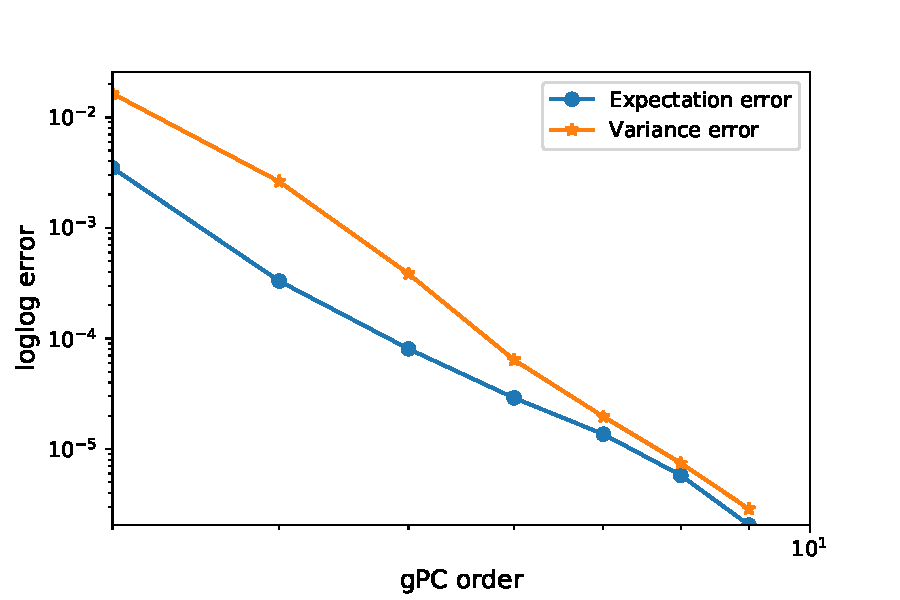
\includegraphics[width=0.5\textwidth]{gPC_hyp/loglog_conv}
  \bicaption[2-14]{例二:初值(\ref{ex2-init1}),二阶离散gPC-SG方法的收敛性,$\ell^1$误差与gPC阶数的关系图(左)和相应的对数图(右)。}{例二:初值(\ref{ex2-init1}),二阶离散gPC-SG方法的收敛性,$\ell^1$误差与gPC阶数的关系图(左)和相应的对数图(右)。}{Fig}{Example 2 with initial data (\ref{ex2-init1}). Convergence of the new gPC-SG method using second order finite difference approximation. Left: the $\ell^1$ error versus the gPC order. Right: the gPC error versus the gPC order by a log-log plot (with other numerical parameters fixed).}
  % \label{2-14}
\end{figure}

\section{本章总结与展望}
在本章中,我们研究了带有间断与随机系数的双曲型方程的数值解法。为了克服由解的奇异性导致的gPC-SG方法收敛速度很慢的问题,我们提出了离散gPC-SG方法,利用离散的解具有较好的正则性,进而改进gPC-SG方法的收敛速度。对于对流方程我们进行了收敛性分析与误差估计。同时为了说明方法的有效性,我们对于对流方程与刘维尔方程进行了大量的数值实验。

对于不光滑的、带有不确定性的问题,gPC-SG方法的应用仍然有很多问题没有解决。上述离散gPC-SG方法在高阶格式构造、非线性问题上仍然存在一定困难,同时如何将该方法向更广泛的问题上进行推广仍然需要大量的研究,会作为未来的研究方向之一。

% \begin{remark}
%   For this second order Liouville equation using our gPC scheme, there still exists many challenges in programming where we need to reduce the CPU time technically. The most time consuming part of this program is the ``FOR'' statements and the condition statements in each ``FOR'' loop (which are very slow in languages such as Python and Matlab). So for our numerical examples, we use $3$ tricks to reduce the computation cost:
%   \begin{itemize}
%     \item Most of the reduced cost is due to the special example we use: the discontinuity of potential only happens at one or few points. So for example we have 100 points in $x$ direction and 100 points in $v$-direction, in general case we should run a $100 \times 100$ loop, however, since the Hamilton preserving condition only takes effect at the two points near by the discontinuity point, we only need to run a $2 \times 100$ loop instead of a full $100 \times 100$ loop. All the left points we don’t need to run any ``FOR'' loop, we just use a vectorized formula (standard second order scheme) to iterate and then modified some of the value using the $2 \times 100$ loop.
%     \item Another part is the condition statements ``if'' in every loop, this is also a huge part of total complexity. We need to determine if $v>0$ or $v<0$ and also $v^2 + 2(V^- - V^+) > 0$ such conditions. The trick here is that we don't want to do the ``if'' judgment, instead because we iterate $v$ in an ascending order, we can know at which step $v$ changes sign (\ie just after the 50th step). So using this trick we can make most of judge statements disappear.
%     \item Some of the index change can be pre-computed. For example, for the reflection part, we can compute it before the whole iteration. But for the transmission part, because it needs a linear interpolation we don’t make it pre-computed so far.
%   \end{itemize}
%   By using these tricks, we can reduce the CPU time by 30 times.
% \end{remark}

%\section{Conclusion}
%In this work, we discuss some new results on the convection equation with disc%ontinuous and random wave speed and the Liouville equation with discontinuous %potentials. The numerical results of our new discrete gPC scheme are shown.


% \subsubsection{The numerical results of the standard gPC scheme}
% In this part, to make a comparison, I will provide the results of a ``standard'' gPC method. All the figures has a one to one corresponding with the figures in above section.

% \begin{figure}[htbp]
%   \includegraphics[width=0.5\textwidth]{c_mean}
%   \includegraphics[width=0.5\textwidth]{c_var}
%   \caption{The standard gPC scheme compared with exact solution: $\Delta x = 0.001$, $\Delta t = 0.25\Delta x$, gPC order $N=30$}
% \end{figure}
% Figure 7 is the validation of the method, which we see a little bit sharper at $x=0$ than the relaxation-gPC method. This is due to the relaxation system is a approximation to the original equation. 
% \begin{figure}[htbp]
%   \centering
%   \includegraphics[width=0.8\textwidth]{c_gpc_error}
%   \caption{The $l^1$ error respect to gPC order.}
% \end{figure}

% Figure 8 also shows the error decay respect to gPC order. In the standard gPC method, the error is smaller than the relaxation one. (The same reason as Figure 7.)

% \begin{figure}[htbp]
%   \includegraphics[width=0.5\textwidth]{c_gpc_error_loglog}
%   \includegraphics[width=0.5\textwidth]{c_gpc_error_logy}
%   \caption{The standard gPC scheme error compared with reference solution. Left: a loglog error. Right: a semilog error.}
% \end{figure}

% Next we choose gPC order $N=30$ as reference solution to test the convergence rate. In Figure 9 shows the results, comparing with the relaxation method, the standard gPC method also shows a exponential convergence which is really surprising me. Although the error is a little larger (See Figure 6 for comparison), this seems a contradiction with the convergence theory. For this issue, I will have a fully discussion in the next section.

% \subsection{Standard gPC method with wavelets as basis}
% In this part, to see the strategy of changing basis, I only give one figure to show the convergence rate to compare with Figure 6, Figure 9. In this test we use the Haar wavelets as basis, and all the other configuration is the same as the standard gPC approach. The results are shown in Figure 10

% \begin{figure}[htbp]
%   \includegraphics[width=0.5\textwidth]{c_wavelet_error_loglog}
%   \includegraphics[width=0.5\textwidth]{c_wavelet_error_logy}
%   \caption{The standard gPC scheme using wavelets as basis: $l^1$ error compared with reference solution. Left: a loglog error. Right: a semilog error.}
% \end{figure}

% We can see the results are really bad, the convergence is very slow compared with previous methods.


% \section{Discussion and analysis of the numerical results}
% In this section, I will go further to discuss the issues I find in the numerical tests and the understanding of this problem.

% At first, from the tests, we can verify that the relaxation-gPC method achieves an exponential convergence, this is not surprising as I have mentioned through all this report. Also, the error of this method (compared to the analytic solution) is a little bit larger than the standard gPC method which is, also not surprising, because the relaxation system is only a approximation of the original equation. Only when $\varepsilon$ is very small, this error should be very small.

% At a second glance at the results, a question comes out: why the ``standard" gPC method also seems to achieve the same exponential converge? It seems unusual and quite surprising. Firstly, let me say, the program is absolutely right. Secondly, the analytic solution indeed has singular which means very very bad regularity in random space as shown in Figure 2. So what's wrong? If so, does it mean the relaxation scheme is useless? To answer these questions, I will give a carefully analysis of these schemes. 

% \subsection{Explaination of the results by ``Standard" gPC Galerkin scheme}
% To make things clear, I first try to following the standard procedure and write down the whole scheme. The notations here is basically the same as in Section 2.2.

% In gPC Galerkin method, we seek an approximate solution in the form of gPC expansion, i.e.
% \begin{equation}\label{expansion}
%   u(t,x,z) = \sum_{k=0}^N\hat{u}_k(t,x)P_k(z)
% \end{equation}
% where $P_k(x)$ are orthonormal polynomial bases with weights $\rho(z)$. The expansion coefficients are determined as
% \begin{equation}
%   \hat{u}_k(t,x)=\int u(t,x,z)P_k(z)\rho(z)\,dz
% \end{equation}

% By utilizing the expansion (\ref{expansion}) and employing a Galerkin projection, it is straightforward to verify that the coefficients $\hat{u}_k(x,t)$ satisfy the following system of equations
% \begin{align}\label{system}
%   &\partial_t\hat{u}_m(t,x)+\partial_x(c(x)\hat{u}_m(t,x))+\sum_{k=0}^N a_{k,m}\partial_x\hat{u}_k(t,x)=0 \quad k=0,1,\cdots,N \\
%   &a_{k,m}=\int z P_k(z)P_m(z)\rho(z)\,dz
% \end{align}
% If we denote by $\mathbf{A}$ the $(N+1)\times(N+1)$ matrix whose entries are $\{a_{k,m}\}_{0\leq k,m\leq N}$ and $\mathbf{u}=(\hat u_0,\cdots,\hat u_N)^T$ a vector of length $(N+1)$, then system (\ref{system}) can be written as
% \begin{equation}
%   \partial_t\mathbf{u}+\partial_x[(c(x)\mathbf{I}+\mathbf{A})\mathbf{u}]=0
% \end{equation}

% After the projection we also have the interface condition corresponding to system (\ref{system}) written as
% \begin{equation}
%   (c^+\mathbf{I}+\mathbf{A})\mathbf{u}(t,0^+)=(c^-\mathbf{I}+\mathbf{A})\mathbf{u}(t,0^-).
% \end{equation}

% Then we solve this system using the immersed upwind method. Let the spatial mesh be $x_i=i\Delta x$, where $i\in\mathbb{Z}$, the set of all integers, and $\Delta x$ is the mesh size. Let $t^n=n\Delta t$ be the discrete time where $\Delta t$ is the time step. Let $\mathbf{U}^n_i=\mathbf{U}(t^n,x_i)$ be the numerical approximation of $\mathbf{u}(t^n,x_i)$. The immersed upwind scheme with interface condition is
% \begin{equation}
% \begin{cases}
% \mathbf{U}_i^{n+1}=(1-\mathbf{\lambda}^-)\mathbf{U}_i^n+\mathbf{\lambda}^-\mathbf{U}_{i-1}^n,\quad \mbox{if } i\leq 0, \\
% \mathbf{U}_i^{n+1}=(1-\mathbf{\lambda}^+)\mathbf{U}_i^n+\mathbf{\lambda}^+\mathbf{\rho}\mathbf{U}_{i-1}^n,\quad \mbox{if } i=1, \\
% \mathbf{U}_i^{n+1}=(1-\mathbf{\lambda}^+)\mathbf{U}_i^n+\mathbf{\lambda}^+\mathbf{U}_{i-1}^n,\quad \mbox{if } i\geq 2, 
% \end{cases}
% \end{equation}
% where $\lambda^{+/-}=(c^{+/-}\mathbf{I}+\mathbf{A})\Delta t/\Delta x$ and $\mathbf{\rho}=(c^{+}\mathbf{I}+\mathbf{A})^{-1}(c^{-}\mathbf{I}+\mathbf{A})$.
% If we explicit put $\rho$ into the scheme we get
% \begin{equation}
% \begin{cases}
% \mathbf{U}_i^{n+1}=(1-\mathbf{\lambda}^-)\mathbf{U}_i^n+\mathbf{\lambda}^-\mathbf{U}_{i-1}^n,\quad \mbox{if } i\leq 0, \\
% \mathbf{U}_i^{n+1}=(1-\mathbf{\lambda}^+)\mathbf{U}_i^n+\mathbf{\lambda}^-\mathbf{U}_{i-1}^n,\quad \mbox{if } i=1, \\
% \mathbf{U}_i^{n+1}=(1-\mathbf{\lambda}^+)\mathbf{U}_i^n+\mathbf{\lambda}^+\mathbf{U}_{i-1}^n,\quad \mbox{if } i\geq 2, 
% \end{cases}
% \end{equation}
% Notice the change in the second equation. This is exactly the scheme I use in the numerical tests. 

% For now, it seems there is no problem. But if I derive the scheme in another way: First, we discretize the origin equation (12) using the method in Qi Peng's paper during which I regard the random $z$ as a fixed parameter. One will obtain the following scheme:
% \begin{equation}
% \begin{cases}
% U_i^{n+1}(z) = (1 - \lambda^-(z))U_i^n+\lambda^-(z)U_{i-1}^n,\quad &\mbox{if } i\leq 0, \\
% U_i^{n+1}(z) = (1 - \lambda^+(z))U_i^n+\lambda^-(z)U_{i-1}^n,\quad &\mbox{if } i=1, \\
% U_i^{n+1}(z) = (1 - \lambda^+(z))U_i^n+\lambda^+(z)U_{i-1}^n,\quad &\mbox{if } i\geq 2, 
% \end{cases}
% \end{equation}

% Wait, if one looks at this scheme you will find: Assume $U^n_{i}$ is analytic respect to $z$ for any $i$, after one time step, the resulting $U^{n+1}_{i}$ is still analytic respect to $z$. The reason is $\lambda^{+/-}$ is a analytic function of $z$! Since the initial data is analytic, as the reason above, the discrete solution at any time $t$ should also be analytic respect to $z$.

% And for this discretized system, if one does the usual gPC Galerin method, you will get to the same system as (51) which is used in numerically tests. From this point of view, the exponential convergence is nothing surprising.

% But why by these two ways you sill get the same system (51)? It is impossible, there must be wrong with one of these two ways. After some time of thinking, in my opinion, the problem comes in the first way. When you do Galerkin approach to the original equation, the interface condition (14) can not be also projected into the space in this way. Such a wrong projection leads to a wrong resulting system. (Still needs more time to think about this problem.)

% So it seems this approach can partially explain the numerical results.

% \subsection{How to understand this phenomenon}
% In this section I want to go further, because the results imply that there should be some ``AP'' or ``uniform accuracy'' like structures which occur in kinetic theory.

% Usually in such problem, there exist two direction limits: the first is gPC expansion when $N\rightarrow\infty$; the second is physical mesh let's say $h\rightarrow 0$. Whether these limits can be exchanged is the nature question of such problem.

% For the standard gPC method in literatures, we first consider $N\rightarrow\infty$ and then let $h\rightarrow 0$. For our problem, when you do like this, in the first step due to the singular of the solution, you will get a bad convergence rate. However, if you first do the second ($h\rightarrow 0$) and then do the Galerkin approach ($N\rightarrow\infty$), you will get a satisfactory results as shown in previous sections.

% From numerical analysis point of view, you want to estimate the error between final numerical solution $\mathbf{U}^N_{h}$ and the exact solution $u$ on some norm, you can do this in two different ways:
% \begin{equation}
% ||\mathbf{U}^N_{h}-u||\leq||\mathbf{U}^N_{h}-\mathbf{U}^N||+||\mathbf{U}^N-u||
% \end{equation}
% or
% \begin{equation}
%   ||\mathbf{U}^N_{h}-u||\leq||\mathbf{U}^N_{h}-U_h||+||U_h-u||.
% \end{equation}
% And for our problem if you do as (53), the $||\mathbf{U}^N-u||$ part can not be estimated. If you do in the second way (54), $|U_h-u||$ can be obtained as the same in Qi Peng's paper (that depends on $z$), $||\mathbf{U}^N_{h}-U_h||$ can be obtained in the standard gPC way. 

% If this idea works for our problem, why we need the relaxation scheme? In relaxation-gPC scheme, there exists one more limit: $\varepsilon\rightarrow 0$. The relation between this limit and gPC limit has been studied recently which is called ``Stocahsitic AP''. In our problem we fix $\varepsilon$ and talk about the other limits. For relaxation-gPC scheme, although the $\varepsilon$ makes the error a bit larger, however, in my opinion, it has a very good property which like the uniform accuracy:
% the other two limits can be exchanged with fixed $\varepsilon$. You can get a uniform error estimate for these two approach. This is the main advantage of such schemes.

% So I think for a large area of problems, this concept I give can be available when building the numerical schemes for some stochastic-physic systems especially for hyperbolic systems.

% \section{Conclusion}
% In this report, I discussed some new results on the convection equation with discontinuous and random wave speed. The numerical results of a new relaxation-gPC scheme are shown. A new understanding of the old standard gPC method are discussed. A new concept for a type of schemes called ``uniform accuracy scheme'' for stochastic-physic system is proposed.
% \bibliographystyle{plain}
% \bibliography{gpc_bibtex}



% \begin{thebibliography}{00}

% %% \bibitem{label}
% %% Text of bibliographic item

% %\bibitem{Babuška:2007kvba} I. Babuska, F. Nobile, R. Tempone, A Stochastic Col%location Method for Elliptic Partial Differential Equations with Random Input %Data, SIAM J. Numer. Anal. 45 (2007) 1005-1034. doi:10.1137/050645142.


% \bibitem{Bijl:2013hkba} H. Bijl, D. Lucor, S. Mishra, C. Schwab, Uncertainty Quantification in Computational Fluid Dynamics, Springer, Cham, 2013. doi:10.1007/978-3-319-00885-1.


% \bibitem{Quarteroni:1982bmba} C. Canuto, A. Quarteroni, Approximation results for orthogonal polynomials in Sobolev spaces, Math. Comp. 38 (1982) 67-86. doi:10.1090/S0025-5718-1982-0637287-3.

% \bibitem{Liu:1998faba} H. Choi, J.G. Liu, The reconstruction of upwind fluxes for conservation laws: its behavior in dynamic and steady state calculations, J. Comput. Phys. 144 (1998) 237-256. doi:10.1006/jcph.1998.5970.

% \bibitem{Des} B. Despres, G. Poette, and D. Lucor. Robust uncertainty propagation in systems of conservation laws with the entropy closure method. In
% Uncertainty Quantication in Computational Fluid Dynamics,
% Volume 92 of
% Lect. Notes Comput. Sci. Eng.,  105-149. Springer, Heidelberg, 2013

% \bibitem{GS} R. G. Ghanem and P. D. Spanos. Stochastic Finite Elements: A Spectral Approach. Springer Verlag,
% New York, 1991.

% \bibitem{GX} D. Gottlieb and D. Xiu, Galerkin method for wave equations with
% uncertain coefficients, Comm. Comp. Phys. 3, 505-518, 2008.

% \bibitem{GWZ} Max D. Gunzburger, Clayton G. Webster, and Guannan Zhang. Stochastic finite element
% methods for partial differential equations with random input data. Acta Numer., 23 (2014), 521-650.

% \bibitem{Jin:2009pro} S. Jin, Numerical methods for hyperbolic systems with singular coefficients: well-balanced scheme, Hamiltonian preservation and beyond, Proc. of the 12th International Conference on Hyperbolic Problems: Theory, Numerics, Applications, Univeristy of Maryland, College Park. Proceedings of Symposia in Applied Mathematics Vol 67-1, 93-104, 2009, American Mathematical Society.

% \bibitem{HJX}  J. Hu, S. Jin, and D. Xiu, A stochastic Galerkin method for Hamilton-Jacobi equations with uncertainty, SIAM J. Sci. Comput. 37, A2246-A2269, 2015. 

% \bibitem{Novak:2006cpba} S. Jin, K.A. Novak, A Semiclassical Transport Model for Thin Quantum Barriers, Multiscale Model. Simul. 5 (2006) 1063-1086. doi:10.1137/060653214.

% \bibitem{Qi:2013byba} S. Jin, P. Qi, $\ell^1$-error estimates on the immersed interface upwind scheme for linear convection equations with piecewise constant coefficients: A simple proof, Science China Mathematics 56 (2013), 2773-2782. doi:10.1007/s11425-013-4738-2.

% %\bibitem{Jin:2014ugba} S. Jin, D. Xiu, X. Zhu, Asymptotic-preserving methods f%or hyperbolic and transport equations with random inputs and diffusive scaling%s, J. Comp. Phys. 289 (2015), 35-52.


% \bibitem{Wen:2005ueba} S. Jin, X. Wen, Hamiltonian-preserving schemes for the Liouville equation with discontinuous potentials, Commun. Math. Sci. 3 (2005) 285-315.

% \bibitem{JinWen-wave} S. Jin and X. Wen, Hamiltonian-preserving schemes for the Liouville equation of geometrical optics with partial transmissions and reflections, SIAM J. Num. Anal. 44 (2006), 1801-1828.

% \bibitem{Tadmor:2000jlba} A. Kurganov, E. Tadmor, New High-Resolution Central Schemes for Nonlinear Conservation Laws and Convection Diffusion Equations, J. Comput. Phys. 160, 241-282, (2000). doi:10.1006/jcph.2000.6459.

% \bibitem{LMK} O. P. Le Maitre and O. M. Knio. Spectral Methods for Uncertainty Quantification, Scientific
% Computation, with Applications to Computational Fluid Dynamics. Springer, New York,
% 2010.

% %\bibitem{Maı̂tre:2004joba} O.P. Le Maitre, O.M. Knio, H.N. Najm, R.G. Ghanem, U%ncertainty propagation using Wiener–Haar expansions, J. Comput. Phys. 197 (200%4) 28-57. doi:10.1016/j.jcp.2003.11.033.

% %\bibitem{Maı̂tre:2004ctba} O.P. Le Maitre, H.N. Najm, R.G. Ghanem, O.M. Knio, M%ulti-resolution analysis of Wiener-type uncertainty propagation schemes, J. Co%mput. Phys. 197 (2004) 502-531. doi:10.1016/j.jcp.2003.12.020.

% \bibitem{LeVeque} R.J. LeVeque, Finite Volume Methods for Hyperbolic Problems,
% Cambridge University Press, 2002.

% %\bibitem{Maître:2007iwba} O.P. Le Maitre, H.N. Najm, P.P. Pebay, R.G. Ghanem, %O.M. Knio, Multi‐Resolution‐Analysis Scheme for Uncertainty Quantification in %Chemical Systems, SIAM J. Sci. Comput. ({\bf Jin remark: publication informati%on})  (2007). doi:10.1137/050643118.

% \bibitem{Motamed:2012gsba} M. Motamed, F. Nobile, R. Tempone, A stochastic collocation method for the second order wave equation with a discontinuous random speed, Numer. Math. 123 (2012) 493-536. doi:10.1007/s00211-012-0493-5.

% \bibitem{PIN} M. P. Pettersson, G. Iaccarino and J. Nordstr\"om, Polynomial Chaos Methods for Hyperbolic Differential Equations, Springer, Switzerland, 2015.

% \bibitem{Tadmor:1990vlba} H. Nessyahu, E. Tadmor, Non-oscillatory central differencing for hyperbolic conservation laws, J. Comput. Phys. (1990).

% \bibitem{Zhou:2010gwba} T. Tang, T. Zhou, Convergence Analysis for Stochastic Collocation Methods to Scalar Hyperbolic Equations with a Random Wave Speed, Commun. Comput. Phys, 8.1 (2010) 226-248. doi:10.4208/cicp.060109.130110a.

% \bibitem{Tryoen:2010djba} J. Tryoen, O. Le Maitre, M. Ndjinga, A. Ern, Intrusive Galerkin methods with upwinding for uncertain nonlinear hyperbolic systems, J. Comput. Phys. 229 (2010) 6485-6511. doi:10.1016/j.jcp.2010.05.007.

% \bibitem{XIU:2009imba} D. Xiu, Fast numerical methods for stochastic computations: a review, Comun. Comput. Phys, 5.2-4 (2009) 242-272. doi:10.1016/j.adhoc.2013.06.001.

% \bibitem{Xiu:2010wxba} D. Xiu, Numerical Methods for Stochastic Computations, Princeton University Press, 2010.

% \bibitem{XiuKar} D. Xiu and  G.E. Karniadakis, The Wiener-Askey polynomial chaos for stochastic
% differential equations. SIAM J. Sci. Comput., 24(2002), 619-644.

% \bibitem{Hesthaven:2005iaba} D. Xiu, J.S. Hesthaven, High-Order Collocation Methods for Differential Equations with Random Inputs, SIAM J. Sci. Comput. 27 (2005) 1118-1139. doi:10.1137/040615201.


% %\bibitem{Zhou:2011ivba} T. Zhou, Stochastic Galerkin methods for elliptic inte%rface problems with random input, J. Comput. Appl. Math. 236 (2011) 782-792. d%oi:10.1016/j.cam.2011.05.033.

% \bibitem{Tang:2012ibba} T. Zhou, T. Tang, Convergence Analysis for Spectral Approximation to a Scalar Transport Equation with a Random Wave Speed, J. Comput. Math. 30 (2012) 643-656. doi:10.4208/jcm.1206-m4012.

% %\bibitem{Zheng:2015deba} M. Zheng, B. Rozovsky, G.E. Karniadakis, Adaptive Wic%k--Malliavin Approximation to Nonlinear SPDEs with Discrete Random Variables, %SIAM J. Sci. Comput. 37 (2015) A1872-A1890. doi:10.1137/140975930.

% \end{thebibliography}
% \end{document}

